\documentclass[11pt]{article}
\usepackage[letterpaper,margin=0.9in]{geometry}
\usepackage{amsmath,amssymb}
\usepackage{tikz}
\usetikzlibrary{arrows.meta,positioning}
\usepackage{enumitem}
\usepackage{titlesec}
\usepackage{array}
\usepackage{booktabs}
\usepackage[normalem]{ulem}

\titleformat{\section}{\large\bfseries}{}{0pt}{}
\titlespacing{\section}{0pt}{10pt}{4pt}
\titleformat{\subsection}{\normalsize\bfseries}{}{0pt}{}
\titlespacing{\subsection}{0pt}{6pt}{2pt}

\newcommand{\op}[1]{\mathit{#1}}
\newcommand{\Fnc}{\op{Fnc}} \newcommand{\Inj}{\op{Inj}} \newcommand{\Srj}{\op{Srj}}
\newcommand{\InjFncs}{\op{InjFncs}} \newcommand{\SrjFncs}{\op{SrjFncs}}
\newcommand{\Eqv}{\op{Eqv}} \newcommand{\PO}{\op{PO}} \newcommand{\DG}{\op{DG}}
\newcommand{\HsDgrm}{\op{HsDgrm}} \newcommand{\EqvClsr}{\op{EqvClsr}} \newcommand{\SymClsr}{\op{SymClsr}} \newcommand{\EqvCls}{\op{EqvCls}}
\newcommand{\TrnsClsr}{\op{TrnsClsr}} \newcommand{\FlxClsr}{\op{FlxClsr}} \newcommand{\Img}{\op{Im}}
\newcommand{\PrtOrdrs}{\op{PrtOrdrs}} \newcommand{\TtlOrdrs}{\op{TtlOrdrs}} \newcommand{\EqvRlns}{\op{EqvRlns}}
\newcommand{\Prtns}{\op{Prtns}}
\newcommand{\mnm}{\operatorname*{mnm}} \newcommand{\mxm}{\operatorname*{mxm}}
\newcommand{\circy}{\fbox{Y}} \newcommand{\circn}{\fbox{N}}
\newcommand{\seclabel}[1]{\noindent\fbox{\textbf{#1}}\par\smallskip}
\tikzset{box/.style={draw,rectangle,minimum width=6mm,minimum height=6mm}}
\newcommand{\radcol}[3]{\foreach \v [count=\i from 0] in {4,3,2,1,0}{\node[box] (#3\v) at (#1,1.6-0.8*\i) {\v};} \node at (#1,2.2) {#2};}
\newcommand{\longdiv}[5]{%
  \begin{tikzpicture}[baseline=-0.5ex,scale=0.62]
    \node at (0.95,0.95) {\footnotesize #3};
    \draw (0,0) -- (0,0.72);
    \draw (0,0.72) -- (2.0,0.72);
    \node at (-0.35,0.15) {\footnotesize #1};
    \node at (1.0,0.35) {\footnotesize #2};
    \node at (1.0,-0.25) {\footnotesize $-$#4};
    \draw (0.45,-0.55) -- (1.55,-0.55);
    \node at (1.0,-0.9) {\footnotesize #5};
  \end{tikzpicture}%
}

\title{\vspace{-1.5cm}Math 163 --- Exam 1B --- Fully Worked Solutions\\
\normalsize J-number 00499317 --- every diagram drawn, every computation shown longhand}
\date{}

\begin{document}
\maketitle
\vspace{-0.7cm}

\section*{0. Setup --- deriving your personal constants}

\subsection*{0.1 Digits of the J-number}
J-number $=00499317$. Reading left to right, $J_1,\dots,J_8$ are just the 8 digits:
\begin{center}
\begin{tabular}{c|cccccccc}
$k$ & 1 & 2 & 3 & 4 & 5 & 6 & 7 & 8\\\hline
$J_k$ & 0 & 0 & 4 & 9 & 9 & 3 & 1 & 7
\end{tabular}
\end{center}

\subsection*{0.2 $r_k := J_k \bmod 5$ --- long division (bus-stop form)}
D\quad $r_k :=$ the remainder obtained upon dividing $J_k$ by $5$.
\begin{center}
\begin{tabular}{cccc}
\longdiv{5}{0}{0}{0}{0} & \longdiv{5}{0}{0}{0}{0} & \longdiv{5}{4}{0}{0}{4} & \longdiv{5}{9}{1}{5}{4}\\
$J_1$ & $J_2$ & $J_3$ & $J_4$\\[4mm]
\longdiv{5}{9}{1}{5}{4} & \longdiv{5}{3}{0}{0}{3} & \longdiv{5}{1}{0}{0}{1} & \longdiv{5}{7}{1}{5}{2}\\
$J_5$ & $J_6$ & $J_7$ & $J_8$
\end{tabular}
\end{center}
The remainder upon dividing $J_1=0$ by $5$ is $0$; hence $r_1=0$. The remainder upon dividing $J_2=0$ by $5$ is $0$; hence $r_2=0$. The remainder upon dividing $J_3=4$ by $5$ is $4$; hence $r_3=4$. The remainder upon dividing $J_4=9$ by $5$ is $4$; hence $r_4=4$. The remainder upon dividing $J_5=9$ by $5$ is $4$; hence $r_5=4$. The remainder upon dividing $J_6=3$ by $5$ is $3$; hence $r_6=3$. The remainder upon dividing $J_7=1$ by $5$ is $1$; hence $r_7=1$. The remainder upon dividing $J_8=7$ by $5$ is $2$; hence $r_8=2$.
\[
r_1=0,\quad r_2=0,\quad r_3=4,\quad r_4=4,\quad r_5=4,\quad r_6=3,\quad r_7=1,\quad r_8=2
\]

\subsection*{0.3 $\op{Prm}(k)$ for $k=1,\dots,8$ --- trial division}
To test if $k$ is prime, divide by every integer from 2 up to $\lfloor\sqrt{k}\rfloor$; if none divide evenly, $k$ is prime ($k\ge2$). $k=1$ needs no trial division at all --- by definition $1$ is \emph{never} prime.
\[
\begin{array}{ll}
k=1: & \text{not prime (by definition, } 1 \text{ is excluded)}\\
k=2: & \lfloor\sqrt2\rfloor=1,\ \text{no divisor to test} \Rightarrow \textbf{prime}\\
k=3: & \lfloor\sqrt3\rfloor=1,\ \text{no divisor to test} \Rightarrow \textbf{prime}\\
k=4: & \lfloor\sqrt4\rfloor=2,\ 4\div2=2\text{ r}0 \Rightarrow \text{divisible} \Rightarrow \text{not prime}\\
k=5: & \lfloor\sqrt5\rfloor=2,\ 5\div2=2\text{ r}1 \Rightarrow \text{no divisor found} \Rightarrow \textbf{prime}\\
k=6: & \lfloor\sqrt6\rfloor=2,\ 6\div2=3\text{ r}0 \Rightarrow \text{divisible} \Rightarrow \text{not prime}\\
k=7: & \lfloor\sqrt7\rfloor=2,\ 7\div2=3\text{ r}1 \Rightarrow \text{no divisor found} \Rightarrow \textbf{prime}\\
k=8: & \lfloor\sqrt8\rfloor=2,\ 8\div2=4\text{ r}0 \Rightarrow \text{divisible} \Rightarrow \text{not prime}
\end{array}
\]
\noindent Recording each test as a circled-choice grid, matching the exam's own $Prm(k)$ table format:
\begin{center}
\begin{tabular}{c|cccccccc}
$k$ & 1 & 2 & 3 & 4 & 5 & 6 & 7 & 8\\\hline
$J_k$ & 0 & 0 & 4 & 9 & 9 & 3 & 1 & 7\\\hline
$Prm(k)=Y$ & N & \fbox{Y} & \fbox{Y} & N & \fbox{Y} & N & \fbox{Y} & N\\
$Prm(k)=N$ & \fbox{N} & N & N & \fbox{N} & N & \fbox{N} & N & \fbox{N}
\end{tabular}
\end{center}
So $\{k\in1..8 \mid \op{Prm}(k)\} = \{2,3,5,7\}$.

\subsection*{0.4 Building $E$, $s$, $b$, $A$, $B$, $R$}

\noindent\textbf{R}\quad For each of the sets defined below, write the elements in increasing order.

\vspace{2mm}
\noindent\textbf{D}\quad Define $\mathcal{U} := 0..9 = \{0,1,2,3,4,5,6,7,8,9\}$.

\vspace{2mm}
\noindent\textbf{D}\quad Define $J := \{J_k\in0..9 \mid k\in1..8\} = \{0,1,3,4,7,9\}$ (the eight digits $0,0,4,9,9,3,1,7$, deduplicated and sorted increasing).

\vspace{2mm}
\noindent\textbf{D}\quad Define $\forall n\in\mathbb{N}\quad \op{Prm}(n) :\Leftrightarrow n\text{ is a prime number}$.

\vspace{2mm}
\noindent\textbf{D}\quad Define
\[
E \ :=\ \{J_k\in0..9 \mid \op{Prm}(k)\} \ =\ \{J_2,J_3,J_5,J_7\} \ =\ \{0,4,9,1\} \ =\ \{0,1,4,9\}
\]
using the $\op{Prm}(k)$ determination from \textbf{0.3}: the prime indices are $k=2,3,5,7$, giving $J_2=0,\ J_3=4,\ J_5=9,\ J_7=1$; sorted increasing, $E=\{0,1,4,9\}$.

\vspace{2mm}
\noindent\textbf{D}\quad $s \ :=\ \mnm_{k\in1..8}\{J_k\in0..9 \mid J_k\neq0\}$.
\[
\{J_3,J_4,J_5,J_6,J_7,J_8\} = \{4,9,9,3,1,7\},\qquad \text{minimum attained at } k=7\ (J_7=1) \ \Rightarrow\ s=1
\]

\vspace{2mm}
\noindent\textbf{D}\quad $b \ :=\ \mxm_{k\in1..8}\{J_k\in0..9 \mid k\in1..8\}+1$. All eight digits are $\{0,0,4,9,9,3,1,7\}$; their maximum is $9$ (attained at $k=4$ and $k=5$), so $b=9+1=10$.

\vspace{2mm}
\noindent\textbf{D}\quad Define
\[
A \ :=\ \{0,s,b\} \ =\ \{0,1,10\}
\]

\vspace{2mm}
\noindent\textbf{D}\quad Define
\[
B \ :=\ \{J_k\in0..9 \mid \op{Prm}(k)\} \ =\ \{0,1,4,9\}\quad(=E, \text{ same defining formula})
\]

\vspace{2mm}
\noindent\textbf{R}\quad Note that in a set an element may occur exactly once, so there are no repeated elements in either $A$ or $B$ above. $A$ and $B$ recur throughout the exam, so any error in these two sets propagates to every later answer.

\vspace{4mm}
\noindent\textbf{D}\quad Define a relation $R\subseteq\{0,1,2,3,4\}\times\{0,1,2,3,4\}=:\mathcal{U}$ by
\[
R \ :=\ \{(0,0)\} \cup \bigcup_{k\in1..4}\{(r_{1+k},r_{2+k})\} \ =\ \{(0,0)\}\cup\{(r_2,r_3),(r_3,r_4),(r_4,r_5),(r_5,r_6)\}
\]
Substituting $r_2=0,\ r_3=4,\ r_4=4,\ r_5=4,\ r_6=3$ from \textbf{0.2}:
\[
R \ =\ \{(0,0)\}\cup\{(0,4),(4,4),(4,4),(4,3)\} \ =\ \{(0,0),(0,4),(4,3),(4,4)\}
\]
(the repeated pair $(4,4)$ only counts once, since $R$ is a \emph{set}.)

\clearpage
\section*{1(abc) --- the relation $R$ on $\{0,1,2,3,4\}$}

\subsection*{(i) Digraph $DG(R)$}
\seclabel{1abc.i}
\begin{center}
\begin{tikzpicture}[every node/.style={draw,circle,minimum size=8mm},>=Stealth,scale=1.1,every node/.append style={transform shape}]
  \node (n0) at (234:2.2cm) {0}; \node (n1) at (306:2.2cm) {1}; \node (n2) at (18:2.2cm) {2};
  \node (n3) at (90:2.2cm) {3}; \node (n4) at (162:2.2cm) {4};
  \draw[->] (n0) edge [loop below, min distance=10mm] (n0);
  \draw[->] (n4) edge [loop left, min distance=10mm] (n4);
  \draw[->] (n0) -- (n4);
  \draw[->] (n4) -- (n3);
\end{tikzpicture}
\end{center}
Vertices $0,\dots,4$ drawn as a pentagon. Self-loops at $0$ and $4$ (from $(0,0),(4,4)$); arrow $0\to4$; arrow $4\to3$; vertices $1,2$ have no edges at all (isolated).

\subsection*{(ii)--(iii) Matrices}
$R^{op}=\{(0,0),(3,4),(4,0),(4,4)\}$. Per the exam's own rule (``in arrow-diagrams, put the numbers in rectangles rather than ovals''), $R$ and $R^{op}$ are first drawn as two-column \textbf{arrow-diagrams} $AD(R)$, $AD(R^{op})$ (domain copy of $\{0,..,4\}$ on the left, codomain copy on the right, elements listed top-to-bottom $4,3,2,1,0$) --- this is the scratch work used to read off each matrix entry.

\seclabel{1abc.ii.0}
\begin{center}
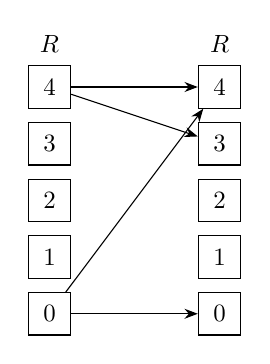
\begin{tikzpicture}[box/.style={draw,rectangle,minimum width=6mm,minimum height=6mm},>=Stealth,scale=0.9,every node/.append style={transform shape}]
  \foreach \v [count=\i from 0] in {4,3,2,1,0} {
    \node[box] (L\v) at (0,1.6-0.8*\i) {\v};
    \node[box] (R\v) at (2.4,1.6-0.8*\i) {\v};
  }
  \node at (0,2.2) {$R$}; \node at (2.4,2.2) {$R$};
  \draw[->] (L0) -- (R0); \draw[->] (L0) -- (R4); \draw[->] (L4) -- (R3); \draw[->] (L4) -- (R4);
\end{tikzpicture}
\end{center}
\centerline{$AD(R)$}

\seclabel{1abc.ii.1}
\noindent $M(R)$, read off $AD(R)$ (row $=$ source, column $=$ target; $1$ if an arrow goes source$\to$target, else $0$): arrows are $L0{\to}R0$, $L0{\to}R4$, $L4{\to}R3$, $L4{\to}R4$, so row $0$ has $1$s at columns $0,4$ and row $4$ has $1$s at columns $3,4$; all other rows are $0$. As a headed grid, then as a bracket matrix:
\begin{center}
\begin{tabular}{c|ccccc}
$M(R)$ & 0&1&2&3&4\\\hline
0 & 1&0&0&0&1\\
1 & 0&0&0&0&0\\
2 & 0&0&0&0&0\\
3 & 0&0&0&0&0\\
4 & 0&0&0&1&1
\end{tabular}
\qquad\qquad
$M(R)=\begin{bmatrix}1&0&0&0&1\\0&0&0&0&0\\0&0&0&0&0\\0&0&0&0&0\\0&0&0&1&1\end{bmatrix}$
\end{center}

\seclabel{1abc.iii.0}
\begin{center}
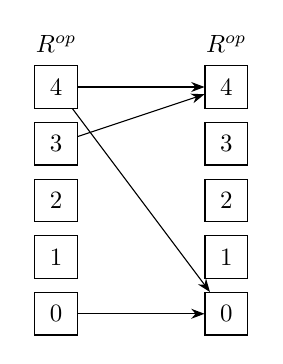
\begin{tikzpicture}[box/.style={draw,rectangle,minimum width=6mm,minimum height=6mm},>=Stealth,scale=0.9,every node/.append style={transform shape}]
  \foreach \v [count=\i from 0] in {4,3,2,1,0} {
    \node[box] (L\v) at (0,1.6-0.8*\i) {\v};
    \node[box] (R\v) at (2.4,1.6-0.8*\i) {\v};
  }
  \node at (0,2.2) {$R^{op}$}; \node at (2.4,2.2) {$R^{op}$};
  \draw[->] (L0) -- (R0); \draw[->] (L3) -- (R4); \draw[->] (L4) -- (R0); \draw[->] (L4) -- (R4);
\end{tikzpicture}
\end{center}
\centerline{$AD(R^{op})$}

\seclabel{1abc.iii.1}
\noindent $M(R^{op})$, read off $AD(R^{op})$: arrows $L0{\to}R0$, $L3{\to}R4$, $L4{\to}R0$, $L4{\to}R4$, so row $0$ has a $1$ at column $0$, row $3$ has a $1$ at column $4$, row $4$ has $1$s at columns $0,4$:
\begin{center}
\begin{tabular}{c|ccccc}
$M(R^{op})$ & 0&1&2&3&4\\\hline
0 & 1&0&0&0&0\\
1 & 0&0&0&0&0\\
2 & 0&0&0&0&0\\
3 & 0&0&0&0&1\\
4 & 1&0&0&0&1
\end{tabular}
\qquad\qquad
$M(R^{op})=\begin{bmatrix}1&0&0&0&0\\0&0&0&0&0\\0&0&0&0&0\\0&0&0&0&1\\1&0&0&0&1\end{bmatrix}$
\end{center}
Rows/columns indexed $0,1,2,3,4$ in order throughout.

\subsection*{(iv) Matrix identities --- shown entry by entry}
\seclabel{1abc.iv.0}
\noindent The two composed relations as their own arrow-diagrams (numbers in rectangles, per the exam's rule):
\begin{center}
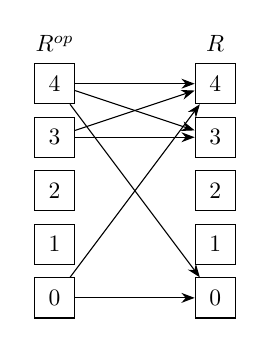
\begin{tikzpicture}[>=Stealth,scale=0.85,every node/.append style={transform shape}]
  \radcol{0}{$R^{op}$}{L}
  \radcol{2.4}{$R$}{R}
  \draw[->] (L0) -- (R0); \draw[->] (L0) -- (R4); \draw[->] (L3) -- (R3); \draw[->] (L3) -- (R4);
  \draw[->] (L4) -- (R0); \draw[->] (L4) -- (R3); \draw[->] (L4) -- (R4);
\end{tikzpicture}
\hspace{1.4cm}
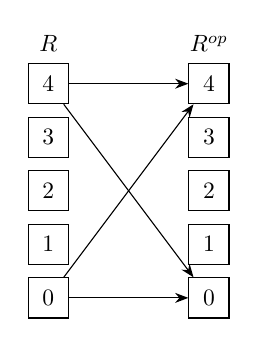
\begin{tikzpicture}[>=Stealth,scale=0.85,every node/.append style={transform shape}]
  \radcol{0}{$R$}{L}
  \radcol{2.4}{$R^{op}$}{R}
  \draw[->] (L0) -- (R0); \draw[->] (L0) -- (R4); \draw[->] (L4) -- (R0); \draw[->] (L4) -- (R4);
\end{tikzpicture}
\end{center}
\centerline{$AD(R\circ R^{op})$ \hspace{5cm} $AD(R^{op}\circ R)$}
Composition convention: $R\circ S := \{(a,c)\mid \exists b,\ (a,b)\in S \wedge (b,c)\in R\}$, so $M(R\circ S) = M(S)\cdot M(R)$ (apply $S$ first).
\[
R\circ R^{op}=\{(0,0),(0,4),(3,3),(3,4),(4,0),(4,3),(4,4)\}, \qquad
R^{op}\circ R=\{(0,0),(0,4),(4,0),(4,4)\}
\]
\begin{center}
\begin{tikzpicture}[every node/.style={draw,circle,minimum size=7mm},>=Stealth,scale=0.95,every node/.append style={transform shape}]
  \node (n0) at (234:2cm) {0}; \node (n1) at (306:2cm) {1}; \node (n2) at (18:2cm) {2};
  \node (n3) at (90:2cm) {3}; \node (n4) at (162:2cm) {4};
  \draw[->] (n0) edge [loop below] (n0);
  \draw[->] (n3) edge [loop above] (n3);
  \draw[->] (n4) edge [loop left] (n4);
  \draw[->] (n0) -- (n4); \draw[->] (n3) -- (n4); \draw[->] (n4) -- (n0); \draw[->] (n4) -- (n3);
\end{tikzpicture}
\hspace{1cm}
\begin{tikzpicture}[every node/.style={draw,circle,minimum size=7mm},>=Stealth,scale=0.95,every node/.append style={transform shape}]
  \node (n0) at (234:2cm) {0}; \node (n1) at (306:2cm) {1}; \node (n2) at (18:2cm) {2};
  \node (n3) at (90:2cm) {3}; \node (n4) at (162:2cm) {4};
  \draw[->] (n0) edge [loop below] (n0);
  \draw[->] (n4) edge [loop left] (n4);
  \draw[->] (n0) -- (n4); \draw[->] (n4) -- (n0);
\end{tikzpicture}
\end{center}
\centerline{$DG(R\circ R^{op})$ \hspace{4.2cm} $DG(R^{op}\circ R)$}

\seclabel{1abc.iv.1}
\noindent\textbf{Identity 1:} $\big(M(R\circ R^{op})\big)(0,1) = \big((M(R^{op}))(M(R))\big)(0,1)$.
\[
\big((M(R^{op}))(M(R))\big)
=\left(\begin{bmatrix}1&0&0&0&0\\0&0&0&0&0\\0&0&0&0&0\\0&0&0&0&1\\1&0&0&0&1\end{bmatrix}\begin{bmatrix}1&0&0&0&1\\0&0&0&0&0\\0&0&0&0&0\\0&0&0&0&0\\0&0&0&1&1\end{bmatrix}\right)
=\begin{bmatrix}a&b&c&d&e\\f&g&h&i&j\\k&l&m&n&o\\p&q&r&s&t\\u&v&w&x&y\end{bmatrix}
\]
Every one of the 25 entries, computed as a full dot-product sum (row of $M(R^{op})$ against column of $M(R)$), labeled $a,\dots,y$ left-to-right, top-to-bottom:
\begingroup\scriptsize
\[
\begin{array}{ll}
a:=(1)(1){+}(0)(0){+}(0)(0){+}(0)(0){+}(0)(0)=1 & b:=(1)(0){+}(0)(0){+}(0)(0){+}(0)(0){+}(0)(0)=0\\
c:=(1)(0){+}(0)(0){+}(0)(0){+}(0)(0){+}(0)(0)=0 & d:=(1)(0){+}(0)(0){+}(0)(0){+}(0)(0){+}(0)(1)=0\\
e:=(1)(1){+}(0)(0){+}(0)(0){+}(0)(0){+}(0)(1)=1 & f:=(0)(1){+}(0)(0){+}(0)(0){+}(0)(0){+}(0)(0)=0\\
g:=(0)(0){+}(0)(0){+}(0)(0){+}(0)(0){+}(0)(0)=0 & h:=(0)(0){+}(0)(0){+}(0)(0){+}(0)(0){+}(0)(0)=0\\
i:=(0)(0){+}(0)(0){+}(0)(0){+}(0)(0){+}(0)(1)=0 & j:=(0)(1){+}(0)(0){+}(0)(0){+}(0)(0){+}(0)(1)=0\\
k:=(0)(1){+}(0)(0){+}(0)(0){+}(0)(0){+}(0)(0)=0 & l:=(0)(0){+}(0)(0){+}(0)(0){+}(0)(0){+}(0)(0)=0\\
m:=(0)(0){+}(0)(0){+}(0)(0){+}(0)(0){+}(0)(0)=0 & n:=(0)(0){+}(0)(0){+}(0)(0){+}(0)(0){+}(0)(1)=0\\
o:=(0)(1){+}(0)(0){+}(0)(0){+}(0)(0){+}(0)(1)=0 & p:=(0)(1){+}(0)(0){+}(0)(0){+}(0)(0){+}(1)(0)=0\\
q:=(0)(0){+}(0)(0){+}(0)(0){+}(0)(0){+}(1)(0)=0 & r:=(0)(0){+}(0)(0){+}(0)(0){+}(0)(0){+}(1)(0)=0\\
s:=(0)(0){+}(0)(0){+}(0)(0){+}(0)(0){+}(1)(1)=1 & t:=(0)(1){+}(0)(0){+}(0)(0){+}(0)(0){+}(1)(1)=1\\
u:=(1)(1){+}(0)(0){+}(0)(0){+}(0)(0){+}(1)(0)=1 & v:=(1)(0){+}(0)(0){+}(0)(0){+}(0)(0){+}(1)(0)=0\\
w:=(1)(0){+}(0)(0){+}(0)(0){+}(0)(0){+}(1)(0)=0 & x:=(1)(0){+}(0)(0){+}(0)(0){+}(0)(0){+}(1)(1)=1\\
y:=(1)(1){+}(0)(0){+}(0)(0){+}(0)(0){+}(1)(1)=2 &
\end{array}
\]
\endgroup
\[
\big((M(R^{op}))(M(R))\big)(0,1)
=\begin{bmatrix}1&0&0&0&1\\0&0&0&0&0\\0&0&0&0&0\\0&0&0&1&1\\1&0&0&1&\mathbf2\end{bmatrix}(0,1)
=\begin{bmatrix}1&0&0&0&1\\0&0&0&0&0\\0&0&0&0&0\\0&0&0&1&1\\1&0&0&1&1\end{bmatrix}
\]

\seclabel{1abc.iv.2}
\noindent As a headed grid, then bracket, $M(R\circ R^{op})$ (read directly off $DG(R\circ R^{op})$ / $AD(R\circ R^{op})$):
\begin{center}
\begin{tabular}{c|ccccc}
$M(R\circ R^{op})$ & 0&1&2&3&4\\\hline
0 & 1&0&0&0&1\\
1 & 0&0&0&0&0\\
2 & 0&0&0&0&0\\
3 & 0&0&0&1&1\\
4 & 1&0&0&1&1
\end{tabular}
\qquad
$M(R\circ R^{op})=\begin{bmatrix}1&0&0&0&1\\0&0&0&0&0\\0&0&0&0&0\\0&0&0&1&1\\1&0&0&1&1\end{bmatrix}$
\end{center}
\[
\text{LS}=\begin{bmatrix}1&0&0&0&1\\0&0&0&0&0\\0&0&0&0&0\\0&0&0&1&1\\1&0&0&1&1\end{bmatrix}=\text{RS}
\]
\centerline{LS $=$ RS}

\seclabel{1abc.iv.3}
\noindent\textbf{Identity 2:} $\big(M(R^{op}\circ R)\big)(0,1) = \big((M(R))(M(R^{op}))\big)(0,1)$.
\[
\big((M(R))(M(R^{op}))\big)
=\left(\begin{bmatrix}1&0&0&0&1\\0&0&0&0&0\\0&0&0&0&0\\0&0&0&0&0\\0&0&0&1&1\end{bmatrix}\begin{bmatrix}1&0&0&0&0\\0&0&0&0&0\\0&0&0&0&0\\0&0&0&0&1\\1&0&0&0&1\end{bmatrix}\right)
=\begin{bmatrix}a&b&c&d&e\\f&g&h&i&j\\k&l&m&n&o\\p&q&r&s&t\\u&v&w&x&y\end{bmatrix}
\]
\begingroup\scriptsize
\[
\begin{array}{ll}
a:=(1)(1){+}(0)(0){+}(0)(0){+}(0)(0){+}(1)(1)=2 & b:=(1)(0){+}(0)(0){+}(0)(0){+}(0)(0){+}(1)(0)=0\\
c:=(1)(0){+}(0)(0){+}(0)(0){+}(0)(0){+}(1)(0)=0 & d:=(1)(0){+}(0)(0){+}(0)(0){+}(0)(0){+}(1)(0)=0\\
e:=(1)(0){+}(0)(0){+}(0)(0){+}(0)(1){+}(1)(1)=1 & f:=(0)(1){+}(0)(0){+}(0)(0){+}(0)(0){+}(0)(1)=0\\
g:=(0)(0){+}(0)(0){+}(0)(0){+}(0)(0){+}(0)(0)=0 & h:=(0)(0){+}(0)(0){+}(0)(0){+}(0)(0){+}(0)(0)=0\\
i:=(0)(0){+}(0)(0){+}(0)(0){+}(0)(0){+}(0)(0)=0 & j:=(0)(0){+}(0)(0){+}(0)(0){+}(0)(1){+}(0)(1)=0\\
k:=(0)(1){+}(0)(0){+}(0)(0){+}(0)(0){+}(0)(1)=0 & l:=(0)(0){+}(0)(0){+}(0)(0){+}(0)(0){+}(0)(0)=0\\
m:=(0)(0){+}(0)(0){+}(0)(0){+}(0)(0){+}(0)(0)=0 & n:=(0)(0){+}(0)(0){+}(0)(0){+}(0)(0){+}(0)(0)=0\\
o:=(0)(0){+}(0)(0){+}(0)(0){+}(0)(1){+}(0)(1)=0 & p:=(0)(1){+}(0)(0){+}(0)(0){+}(0)(0){+}(0)(1)=0\\
q:=(0)(0){+}(0)(0){+}(0)(0){+}(0)(0){+}(0)(0)=0 & r:=(0)(0){+}(0)(0){+}(0)(0){+}(0)(0){+}(0)(0)=0\\
s:=(0)(0){+}(0)(0){+}(0)(0){+}(0)(0){+}(0)(0)=0 & t:=(0)(0){+}(0)(0){+}(0)(0){+}(0)(1){+}(0)(1)=0\\
u:=(0)(1){+}(0)(0){+}(0)(0){+}(1)(0){+}(1)(1)=1 & v:=(0)(0){+}(0)(0){+}(0)(0){+}(1)(0){+}(1)(0)=0\\
w:=(0)(0){+}(0)(0){+}(0)(0){+}(1)(0){+}(1)(0)=0 & x:=(0)(0){+}(0)(0){+}(0)(0){+}(1)(0){+}(1)(0)=0\\
y:=(0)(0){+}(0)(0){+}(0)(0){+}(1)(1){+}(1)(1)=2 &
\end{array}
\]
\endgroup
\[
\big((M(R))(M(R^{op}))\big)(0,1)
=\begin{bmatrix}\mathbf2&0&0&0&1\\0&0&0&0&0\\0&0&0&0&0\\0&0&0&0&0\\1&0&0&0&\mathbf2\end{bmatrix}(0,1)
=\begin{bmatrix}1&0&0&0&1\\0&0&0&0&0\\0&0&0&0&0\\0&0&0&0&0\\1&0&0&0&1\end{bmatrix}
\]

\seclabel{1abc.iv.4}
\noindent As a headed grid, then bracket, $M(R^{op}\circ R)$:
\begin{center}
\begin{tabular}{c|ccccc}
$M(R^{op}\circ R)$ & 0&1&2&3&4\\\hline
0 & 1&0&0&0&1\\
1 & 0&0&0&0&0\\
2 & 0&0&0&0&0\\
3 & 0&0&0&0&0\\
4 & 1&0&0&0&1
\end{tabular}
\qquad
$M(R^{op}\circ R)=\begin{bmatrix}1&0&0&0&1\\0&0&0&0&0\\0&0&0&0&0\\0&0&0&0&0\\1&0&0&0&1\end{bmatrix}$
\end{center}
\[
\text{LS}=\begin{bmatrix}1&0&0&0&1\\0&0&0&0&0\\0&0&0&0&0\\0&0&0&0&0\\1&0&0&0&1\end{bmatrix}=\text{RS}
\]
\centerline{LS $=$ RS}

\clearpage
\subsection*{(v) $\FlxClsr(R)$ --- reflexive closure}
\seclabel{1abc.v.0}
\begin{center}
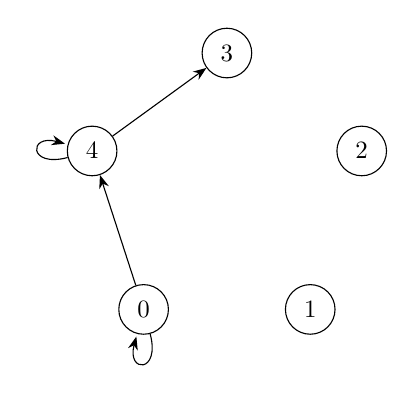
\begin{tikzpicture}[every node/.style={draw,circle,minimum size=7mm},>=Stealth,scale=0.9,every node/.append style={transform shape}]
  \node (n0) at (234:2cm) {0}; \node (n1) at (306:2cm) {1}; \node (n2) at (18:2cm) {2};
  \node (n3) at (90:2cm) {3}; \node (n4) at (162:2cm) {4};
  \draw[->] (n0) edge [loop below] (n0); \draw[->] (n4) edge [loop left] (n4);
  \draw[->] (n0) -- (n4); \draw[->] (n4) -- (n3);
\end{tikzpicture}
\hspace{1.2cm}
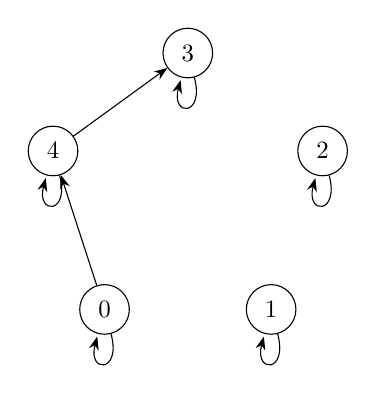
\begin{tikzpicture}[every node/.style={draw,circle,minimum size=7mm},>=Stealth,scale=0.9,every node/.append style={transform shape}]
  \node (n0) at (234:2cm) {0}; \node (n1) at (306:2cm) {1}; \node (n2) at (18:2cm) {2};
  \node (n3) at (90:2cm) {3}; \node (n4) at (162:2cm) {4};
  \foreach \n in {n0,n1,n2,n3,n4} \draw[->] (\n) edge [loop below] (\n);
  \draw[->] (n0) -- (n4); \draw[->] (n4) -- (n3);
\end{tikzpicture}
\end{center}
\centerline{$DG(R)$ \hspace{4.5cm} $DG(\FlxClsr(R))$}

\seclabel{1abc.v.1}
$\FlxClsr(R)$, read directly off $DG(\FlxClsr(R))$ by adding a self-loop at every vertex that lacks one:
\[
\FlxClsr(R) = \{(0,0),(0,4),(1,1),(2,2),(3,3),(4,3),(4,4)\}
\]

\seclabel{1abc.v.2}
$\big(M(\FlxClsr(R))\big)(0,1)$:
\begin{center}
\begin{tabular}{c|ccccc}
& 0&1&2&3&4\\\hline
0 & 1&0&0&0&1\\
1 & 0&1&0&0&0\\
2 & 0&0&1&0&0\\
3 & 0&0&0&1&0\\
4 & 0&0&0&1&1
\end{tabular}
\qquad
$\big(M(\FlxClsr(R))\big)(0,1)=\begin{bmatrix}1&0&0&0&1\\0&1&0&0&0\\0&0&1&0&0\\0&0&0&1&0\\0&0&0&1&1\end{bmatrix}$
\end{center}

\seclabel{1abc.v.3}
$\Delta_{\{0,..,4\}} = \{(0,0),(1,1),(2,2),(3,3),(4,4)\}$

\seclabel{1abc.v.4}
\[
R\cup\big(\Delta_{\{0,..,4\}}\big) = \{(0,0),(0,4),(4,3),(4,4)\}\cup\{(0,0),(1,1),(2,2),(3,3),(4,4)\}
\]
\[
= \{(0,0),(0,4),(1,1),(2,2),(3,3),(4,3),(4,4)\}
\]

\seclabel{1abc.v.5}
$\big(M(R\cup(\Delta_{\{0,..,4\}}))\big)(0,1)$:
\begin{center}
\begin{tabular}{c|ccccc}
& 0&1&2&3&4\\\hline
0 & 1&0&0&0&1\\
1 & 0&1&0&0&0\\
2 & 0&0&1&0&0\\
3 & 0&0&0&1&0\\
4 & 0&0&0&1&1
\end{tabular}
\qquad
$\big(M(R\cup(\Delta_{\{0,..,4\}}))\big)(0,1)=\begin{bmatrix}1&0&0&0&1\\0&1&0&0&0\\0&0&1&0&0\\0&0&0&1&0\\0&0&0&1&1\end{bmatrix}$
\end{center}

\noindent\textbf{Prove:} $\big(M(\FlxClsr(R))\big)(0,1) = \big(M(R\cup(\Delta_{\{0,..,4\}}))\big)(0,1)$.
\[
\text{LS}=\begin{bmatrix}1&0&0&0&1\\0&1&0&0&0\\0&0&1&0&0\\0&0&0&1&0\\0&0&0&1&1\end{bmatrix}=\text{RS}
\]
\centerline{LS $=$ RS}

\subsection*{(vi) $\SymClsr(R)$ --- symmetric closure}
\seclabel{1abc.vi.0}
\begin{center}
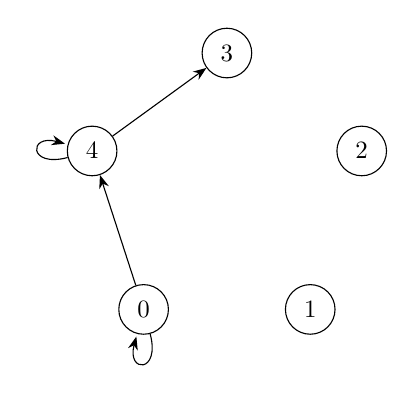
\begin{tikzpicture}[every node/.style={draw,circle,minimum size=7mm},>=Stealth,scale=0.9,every node/.append style={transform shape}]
  \node (n0) at (234:2cm) {0}; \node (n1) at (306:2cm) {1}; \node (n2) at (18:2cm) {2};
  \node (n3) at (90:2cm) {3}; \node (n4) at (162:2cm) {4};
  \draw[->] (n0) edge [loop below] (n0); \draw[->] (n4) edge [loop left] (n4);
  \draw[->] (n0) -- (n4); \draw[->] (n4) -- (n3);
\end{tikzpicture}
\hspace{1.2cm}
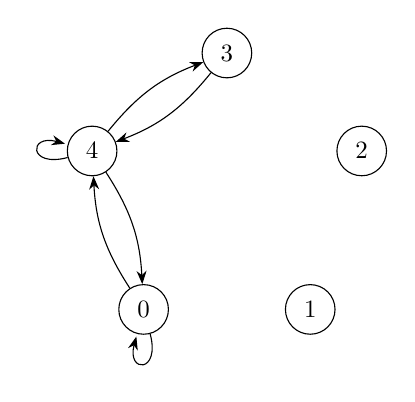
\begin{tikzpicture}[every node/.style={draw,circle,minimum size=7mm},>=Stealth,scale=0.9,every node/.append style={transform shape}]
  \node (n0) at (234:2cm) {0}; \node (n1) at (306:2cm) {1}; \node (n2) at (18:2cm) {2};
  \node (n3) at (90:2cm) {3}; \node (n4) at (162:2cm) {4};
  \draw[->] (n0) edge [loop below] (n0); \draw[->] (n4) edge [loop left] (n4);
  \draw[->] (n0) edge[bend left=15] (n4); \draw[->] (n4) edge[bend left=15] (n0);
  \draw[->] (n4) edge[bend left=15] (n3); \draw[->] (n3) edge[bend left=15] (n4);
\end{tikzpicture}
\end{center}
\centerline{$DG(R)$ \hspace{4.5cm} $DG(\SymClsr(R))$}

\seclabel{1abc.vi.1}
$\SymClsr(R)$, read off $DG(\SymClsr(R))$ by adding the reverse of every edge that lacks a matching reverse:
\[
\SymClsr(R) = \{(0,0),(0,4),(3,4),(4,0),(4,3),(4,4)\}
\]

\seclabel{1abc.vi.2}
$\big(M(\SymClsr(R))\big)(0,1)$:
\begin{center}
\begin{tabular}{c|ccccc}
& 0&1&2&3&4\\\hline
0 & 1&0&0&0&1\\
1 & 0&0&0&0&0\\
2 & 0&0&0&0&0\\
3 & 0&0&0&0&1\\
4 & 1&0&0&1&1
\end{tabular}
\qquad
$=\begin{bmatrix}1&0&0&0&1\\0&0&0&0&0\\0&0&0&0&0\\0&0&0&0&1\\1&0&0&1&1\end{bmatrix}$
\end{center}

\seclabel{1abc.vi.3}
\[
R\cup(R^{op}) = \{(0,0),(0,4),(4,3),(4,4)\}\cup\{(0,0),(3,4),(4,0),(4,4)\}
\]
\[
= \{(0,0),(0,4),(3,4),(4,0),(4,3),(4,4)\}
\]

\seclabel{1abc.vi.4}
$\big(M(R\cup(R^{op}))\big)(0,1)$:
\begin{center}
\begin{tabular}{c|ccccc}
& 0&1&2&3&4\\\hline
0 & 1&0&0&0&1\\
1 & 0&0&0&0&0\\
2 & 0&0&0&0&0\\
3 & 0&0&0&0&1\\
4 & 1&0&0&1&1
\end{tabular}
\qquad
$\big(M(R\cup(R^{op}))\big)(0,1)=\begin{bmatrix}1&0&0&0&1\\0&0&0&0&0\\0&0&0&0&0\\0&0&0&0&1\\1&0&0&1&1\end{bmatrix}$
\end{center}

\noindent\textbf{Prove:} $\big(M(\SymClsr(R))\big)(0,1) = \big(M(R\cup(R^{op}))\big)(0,1)$.
\[
\text{LS}=\begin{bmatrix}1&0&0&0&1\\0&0&0&0&0\\0&0&0&0&0\\0&0&0&0&1\\1&0&0&1&1\end{bmatrix}=\text{RS}
\]
\centerline{LS $=$ RS}

\clearpage
\subsection*{(vii) $\TrnsClsr(R)$ --- transitive closure, powers via arrow-diagram chase}
\seclabel{1abc.vii.0}
\begin{center}
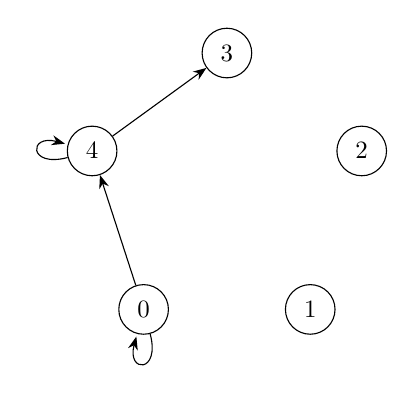
\begin{tikzpicture}[every node/.style={draw,circle,minimum size=7mm},>=Stealth,scale=0.9,every node/.append style={transform shape}]
  \node (n0) at (234:2cm) {0}; \node (n1) at (306:2cm) {1}; \node (n2) at (18:2cm) {2};
  \node (n3) at (90:2cm) {3}; \node (n4) at (162:2cm) {4};
  \draw[->] (n0) edge [loop below] (n0); \draw[->] (n4) edge [loop left] (n4);
  \draw[->] (n0) -- (n4); \draw[->] (n4) -- (n3);
\end{tikzpicture}
\hspace{1.2cm}
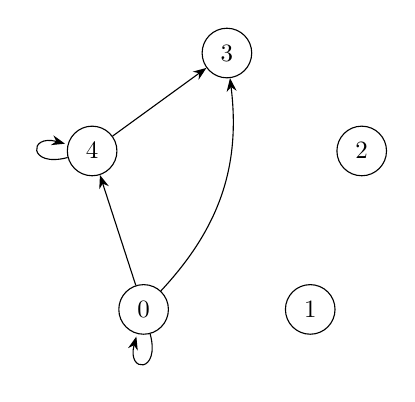
\begin{tikzpicture}[every node/.style={draw,circle,minimum size=7mm},>=Stealth,scale=0.9,every node/.append style={transform shape}]
  \node (n0) at (234:2cm) {0}; \node (n1) at (306:2cm) {1}; \node (n2) at (18:2cm) {2};
  \node (n3) at (90:2cm) {3}; \node (n4) at (162:2cm) {4};
  \draw[->] (n0) edge [loop below] (n0); \draw[->] (n4) edge [loop left] (n4);
  \draw[->] (n0) -- (n4); \draw[->] (n4) -- (n3); \draw[->] (n0) edge[bend right=25] (n3);
\end{tikzpicture}
\end{center}
\centerline{$DG(R)$ \hspace{4.5cm} $DG(\TrnsClsr(R))$}

We compute $R^{\circ k}:=R^{\circ(k-1)}\circ R$ for $k=1,\dots,5$ (with $R^{\circ0}:=\Delta_{\{0,..,4\}}$), each power found by an \textbf{arrow-diagram chase} rather than numeric matrix multiplication: draw $R$ (left column $\to$ middle column) and $R^{\circ(k-1)}$ (middle column $\to$ right column) side by side, then read off $R^{\circ k}$ as every left-to-right pair reachable via some middle vertex.

\seclabel{1abc.vii.1}
\noindent $k=1$: $R^{\circ1}=R^{\circ0}\circ R = \Delta_{\{0,..,4\}}\circ R$.
\begin{center}
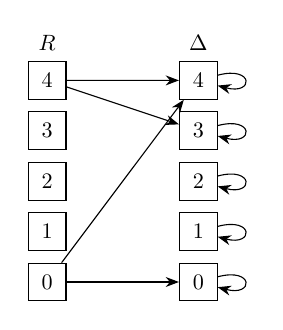
\begin{tikzpicture}[>=Stealth,scale=0.8,every node/.append style={transform shape}]
  \radcol{0}{$R$}{L}
  \radcol{2.4}{$\Delta$}{M}
  \draw[->] (L0) -- (M0); \draw[->] (L0) -- (M4); \draw[->] (L4) -- (M3); \draw[->] (L4) -- (M4);
  \draw[->] (M0) edge[loop right,min distance=6mm] (M0); \draw[->] (M1) edge[loop right,min distance=6mm] (M1); \draw[->] (M2) edge[loop right,min distance=6mm] (M2); \draw[->] (M3) edge[loop right,min distance=6mm] (M3); \draw[->] (M4) edge[loop right,min distance=6mm] (M4);
\end{tikzpicture}
\end{center}
\centerline{$AD(\Delta_{\{0,..,4\}}\circ R)$ --- chasing through the identity changes nothing}
\[
R^{\circ1} = \{(0,0),(0,4),(4,3),(4,4)\}
\]

\seclabel{1abc.vii.2}
\noindent $k=2$: $R^{\circ2}=R^{\circ1}\circ R$.
\begin{center}
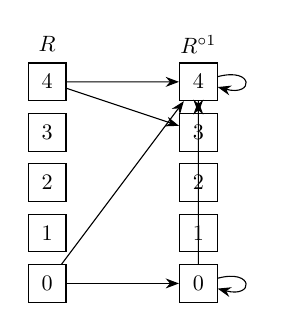
\begin{tikzpicture}[>=Stealth,scale=0.8,every node/.append style={transform shape}]
  \radcol{0}{$R$}{L}
  \radcol{2.4}{$R^{\circ1}$}{M}
  \draw[->] (L0) -- (M0); \draw[->] (L0) -- (M4); \draw[->] (L4) -- (M3); \draw[->] (L4) -- (M4);
  \draw[->] (M0) edge[loop right,min distance=6mm] (M0); \draw[->] (M0) -- (M4); \draw[->] (M4) -- (M3); \draw[->] (M4) edge[loop right,min distance=6mm] (M4);
\end{tikzpicture}
\end{center}
\centerline{$AD(R^{\circ1}\circ R)$}
Chasing: $0\to0\to\{0,4\}$ and $0\to4\to\{3,4\}$, so $0$ reaches $\{0,3,4\}$; $4\to3\to\{\}$ (no arrows leave $3$ in $R^{\circ1}$) and $4\to4\to\{3,4\}$, so $4$ reaches $\{3,4\}$.
\[
R^{\circ2} = \{(0,0),(0,3),(0,4),(4,3),(4,4)\}
\]

\seclabel{1abc.vii.3}
\noindent $k=3$: $R^{\circ3}=R^{\circ2}\circ R$.
\begin{center}
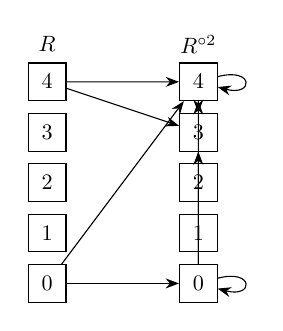
\begin{tikzpicture}[>=Stealth,scale=0.8,every node/.append style={transform shape}]
  \radcol{0}{$R$}{L}
  \radcol{2.4}{$R^{\circ2}$}{M}
  \draw[->] (L0) -- (M0); \draw[->] (L0) -- (M4); \draw[->] (L4) -- (M3); \draw[->] (L4) -- (M4);
  \draw[->] (M0) edge[loop right,min distance=6mm] (M0); \draw[->] (M0) -- (M3); \draw[->] (M0) -- (M4); \draw[->] (M4) -- (M3); \draw[->] (M4) edge[loop right,min distance=6mm] (M4);
\end{tikzpicture}
\end{center}
\centerline{$AD(R^{\circ2}\circ R)$}
Chasing: $0\to0\to\{0,3,4\}$ and $0\to4\to\{3,4\}$, so $0$ reaches $\{0,3,4\}$; $4\to3\to\{\}$ and $4\to4\to\{3,4\}$, so $4$ reaches $\{3,4\}$ --- identical to $R^{\circ2}$.
\[
R^{\circ3} = \{(0,0),(0,3),(0,4),(4,3),(4,4)\} = R^{\circ2}
\]
No new pairs appeared, so the chase has \textbf{stabilized}. Composing an already-stable relation with $R$ again reproduces the same result, so $R^{\circ4}=R^{\circ5}=R^{\circ2}$ as well, without needing to redo the chase.

\seclabel{1abc.vii.4}
\[
R^{\circ4} = R^{\circ3}\circ R = R^{\circ2} = \{(0,0),(0,3),(0,4),(4,3),(4,4)\}
\]
\[
R^{\circ5} = R^{\circ4}\circ R = R^{\circ2} = \{(0,0),(0,3),(0,4),(4,3),(4,4)\}
\]

\seclabel{1abc.vii.5}
\[
\bigcup_{k=1}^{5}R^{\circ k} = R^{\circ1}\cup R^{\circ2}\cup R^{\circ3}\cup R^{\circ4}\cup R^{\circ5} = \{(0,0),(0,3),(0,4),(4,3),(4,4)\}
\]
\noindent\textbf{Why stopping at $k=5$ is enough (pigeonhole):} $\nu(\{0,..,4\})=5$. Any directed path with more than $5$ edges must revisit a vertex, giving a shorter path (delete the cycle) with the same endpoints. So every reachable pair is already reachable by a path of length $\le5$.

\seclabel{1abc.vii.6}
$\big(M(\TrnsClsr(R))\big)(0,1)$ and $\big(M(\bigcup_{k=1}^5 R^{\circ k})\big)(0,1)$:
\begin{center}
\begin{tabular}{c|ccccc}
& 0&1&2&3&4\\\hline
0 & 1&0&0&1&1\\
1 & 0&0&0&0&0\\
2 & 0&0&0&0&0\\
3 & 0&0&0&0&0\\
4 & 1&0&0&1&1
\end{tabular}
\qquad
$=\begin{bmatrix}1&0&0&1&1\\0&0&0&0&0\\0&0&0&0&0\\0&0&0&0&0\\1&0&0&1&1\end{bmatrix}$
\end{center}

\noindent\textbf{Prove:} $\big(M(\TrnsClsr(R))\big)(0,1) = \big(M(\bigcup_{k=1}^5 R^{\circ k})\big)(0,1)$.
\[
\text{LS}=\begin{bmatrix}1&0&0&1&1\\0&0&0&0&0\\0&0&0&0&0\\0&0&0&0&0\\1&0&0&1&1\end{bmatrix}=\text{RS}
\]
\centerline{LS $=$ RS}

\clearpage
\subsection*{(viii) $\EqvClsr(R)$ --- equivalence closure, equivalence classes, quotient}
\seclabel{1abc.viii.0}
\begin{center}
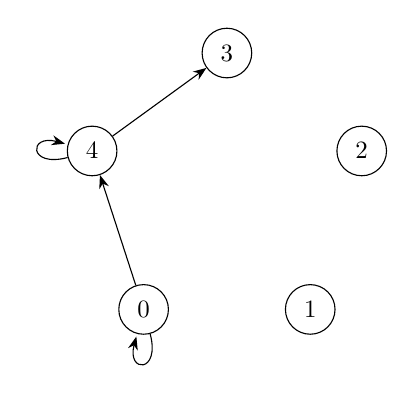
\begin{tikzpicture}[every node/.style={draw,circle,minimum size=7mm},>=Stealth,scale=0.9,every node/.append style={transform shape}]
  \node (n0) at (234:2cm) {0}; \node (n1) at (306:2cm) {1}; \node (n2) at (18:2cm) {2};
  \node (n3) at (90:2cm) {3}; \node (n4) at (162:2cm) {4};
  \draw[->] (n0) edge [loop below] (n0); \draw[->] (n4) edge [loop left] (n4);
  \draw[->] (n0) -- (n4); \draw[->] (n4) -- (n3);
\end{tikzpicture}
\hspace{1cm}
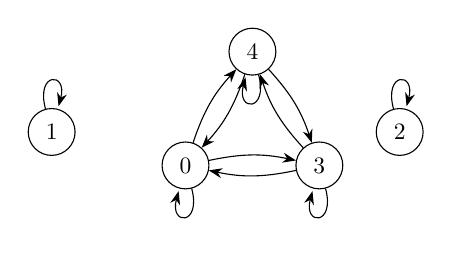
\begin{tikzpicture}[every node/.style={draw,circle,minimum size=7mm},>=Stealth,scale=0.85,every node/.append style={transform shape}]
  \node (n0) at (0,0) {0}; \node (n3) at (2,0) {3}; \node (n4) at (1,1.7) {4};
  \node (n1) at (-2,0.5) {1}; \node (n2) at (3.2,0.5) {2};
  \foreach \n in {n0,n3,n4} \draw[->] (\n) edge [loop below] (\n);
  \draw[->] (n1) edge [loop above] (n1); \draw[->] (n2) edge [loop above] (n2);
  \draw[->] (n0) edge[bend left=12] (n3); \draw[->] (n3) edge[bend left=12] (n0);
  \draw[->] (n0) edge[bend left=12] (n4); \draw[->] (n4) edge[bend left=12] (n0);
  \draw[->] (n3) edge[bend left=12] (n4); \draw[->] (n4) edge[bend left=12] (n3);
\end{tikzpicture}
\end{center}
\centerline{$DG(R)$ \hspace{5.2cm} $DG(\EqvClsr(R))$}

\seclabel{1abc.viii.1}
$\EqvClsr(R)$, read directly off $DG(\EqvClsr(R))$ (the smallest reflexive, symmetric, transitive relation containing $R$ --- every vertex gets a loop, every edge gets its reverse, and $\{0,3,4\}$ close up into a clique since $0,3,4$ are all mutually reachable through $R$):
\[
\EqvClsr(R) = \{(0,0),(0,3),(0,4),(1,1),(2,2),(3,0),(3,3),(3,4),(4,0),(4,3),(4,4)\}
\]

\seclabel{1abc.viii.2}
$\big(M(\EqvClsr(R))\big)(0,1)$:
\begin{center}
\begin{tabular}{c|ccccc}
& 0&1&2&3&4\\\hline
0 & 1&0&0&1&1\\
1 & 0&1&0&0&0\\
2 & 0&0&1&0&0\\
3 & 1&0&0&1&1\\
4 & 1&0&0&1&1
\end{tabular}
\qquad
$\big(M(\EqvClsr(R))\big)(0,1)=\begin{bmatrix}1&0&0&1&1\\0&1&0&0&0\\0&0&1&0&0\\1&0&0&1&1\\1&0&0&1&1\end{bmatrix}$
\end{center}

\seclabel{1abc.viii.3}
\noindent Equivalence class of each element under $\EqvClsr(R)$ (row $x$ of the matrix above, read as a set):
\[
\EqvCls(0,\EqvClsr(R))=\{0,3,4\}, \quad \EqvCls(1,\EqvClsr(R))=\{1\}, \quad \EqvCls(2,\EqvClsr(R))=\{2\},
\]
\[
\EqvCls(3,\EqvClsr(R))=\{0,3,4\}, \quad \EqvCls(4,\EqvClsr(R))=\{0,3,4\}
\]

\seclabel{1abc.viii.4}
\noindent\textbf{Quotient:}
\[
\dfrac{\{0,1,2,3,4\}}{\EqvClsr(R)} = \big\{\EqvCls(x,\EqvClsr(R))\in\mathcal{P}(0..4) \mid x\in\{0,1,2,3,4\}\big\} = \big\{\{0,3,4\},\{1\},\{2\}\big\}
\]
\begin{center}
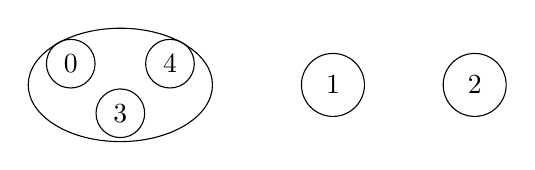
\begin{tikzpicture}[every node/.style={draw,circle,minimum size=6mm},scale=0.9]
  \draw (0,0) ellipse (1.3cm and 0.8cm);
  \node at (-0.7,0.3) {0}; \node at (0,-0.4) {3}; \node at (0.7,0.3) {4};
  \node[draw,circle,minimum size=8mm] (c2) at (3,0) {1};
  \node[draw,circle,minimum size=8mm] (c3) at (5,0) {2};
\end{tikzpicture}
\end{center}
The digraph $DG(\EqvClsr(R))$ splits into 3 disconnected cliques $\{0,3,4\}$, $\{1\}$, $\{2\}$, one per equivalence class.

\clearpage
\subsection*{(ix) $\EqvClsr(R)$ --- powers of $Q:=R\cup R^{op}$ via arrow-diagram chase}
\seclabel{1abc.ix.0}
\begin{center}
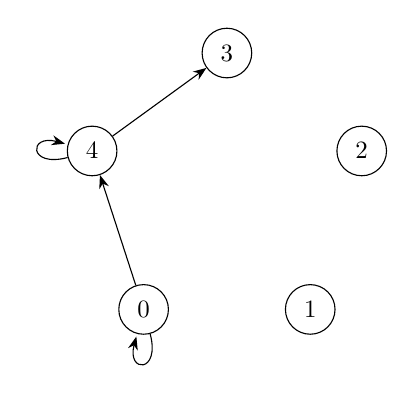
\begin{tikzpicture}[every node/.style={draw,circle,minimum size=7mm},>=Stealth,scale=0.9,every node/.append style={transform shape}]
  \node (n0) at (234:2cm) {0}; \node (n1) at (306:2cm) {1}; \node (n2) at (18:2cm) {2};
  \node (n3) at (90:2cm) {3}; \node (n4) at (162:2cm) {4};
  \draw[->] (n0) edge [loop below] (n0); \draw[->] (n4) edge [loop left] (n4);
  \draw[->] (n0) -- (n4); \draw[->] (n4) -- (n3);
\end{tikzpicture}
\hspace{1cm}
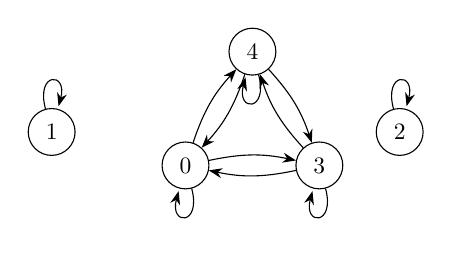
\begin{tikzpicture}[every node/.style={draw,circle,minimum size=7mm},>=Stealth,scale=0.85,every node/.append style={transform shape}]
  \node (n0) at (0,0) {0}; \node (n3) at (2,0) {3}; \node (n4) at (1,1.7) {4};
  \node (n1) at (-2,0.5) {1}; \node (n2) at (3.2,0.5) {2};
  \foreach \n in {n0,n3,n4} \draw[->] (\n) edge [loop below] (\n);
  \draw[->] (n1) edge [loop above] (n1); \draw[->] (n2) edge [loop above] (n2);
  \draw[->] (n0) edge[bend left=12] (n3); \draw[->] (n3) edge[bend left=12] (n0);
  \draw[->] (n0) edge[bend left=12] (n4); \draw[->] (n4) edge[bend left=12] (n0);
  \draw[->] (n3) edge[bend left=12] (n4); \draw[->] (n4) edge[bend left=12] (n3);
\end{tikzpicture}
\end{center}
\centerline{$DG(R)$ \hspace{5.2cm} $DG(\EqvClsr(R))$}

\seclabel{1abc.ix.1}
$\big(M(\EqvClsr(R))\big)(0,1) = \begin{bmatrix}1&0&0&1&1\\0&1&0&0&0\\0&0&1&0&0\\1&0&0&1&1\\1&0&0&1&1\end{bmatrix}$ (from part (viii)).

\seclabel{1abc.ix.2}
\[
R=\{(0,0),(0,4),(4,3),(4,4)\}, \qquad R^{op}=\{(0,0),(3,4),(4,0),(4,4)\}
\]
\[
Q:=R\cup(R^{op}) = \{(0,0),(0,4),(3,4),(4,0),(4,3),(4,4)\}
\]

We compute $Q^{\circ k}:=Q^{\circ(k-1)}\circ Q$ for $k=1,\dots,5$ (with $Q^{\circ0}:=\Delta_{\{0,..,4\}}$), again by \textbf{arrow-diagram chase}, the same method as part (vii).

\seclabel{1abc.ix.3}
\noindent $k=1$: $Q^{\circ1}=Q^{\circ0}\circ Q = \Delta_{\{0,..,4\}}\circ Q$.
\begin{center}
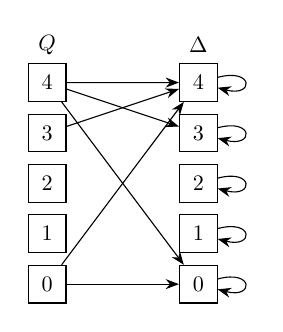
\begin{tikzpicture}[>=Stealth,scale=0.8,every node/.append style={transform shape}]
  \radcol{0}{$Q$}{L}
  \radcol{2.4}{$\Delta$}{M}
  \draw[->] (L0) -- (M0); \draw[->] (L0) -- (M4); \draw[->] (L3) -- (M4); \draw[->] (L4) -- (M0); \draw[->] (L4) -- (M3); \draw[->] (L4) -- (M4);
  \draw[->] (M0) edge[loop right,min distance=6mm] (M0); \draw[->] (M1) edge[loop right,min distance=6mm] (M1); \draw[->] (M2) edge[loop right,min distance=6mm] (M2); \draw[->] (M3) edge[loop right,min distance=6mm] (M3); \draw[->] (M4) edge[loop right,min distance=6mm] (M4);
\end{tikzpicture}
\end{center}
\centerline{$AD(\Delta_{\{0,..,4\}}\circ Q)$ --- chasing through the identity changes nothing}
\[
Q^{\circ1} = \{(0,0),(0,4),(3,4),(4,0),(4,3),(4,4)\}
\]

\seclabel{1abc.ix.4}
\noindent $k=2$: $Q^{\circ2}=Q^{\circ1}\circ Q$.
\begin{center}
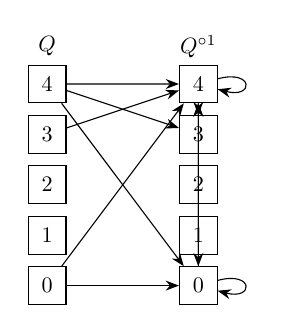
\begin{tikzpicture}[>=Stealth,scale=0.8,every node/.append style={transform shape}]
  \radcol{0}{$Q$}{L}
  \radcol{2.4}{$Q^{\circ1}$}{M}
  \draw[->] (L0) -- (M0); \draw[->] (L0) -- (M4); \draw[->] (L3) -- (M4); \draw[->] (L4) -- (M0); \draw[->] (L4) -- (M3); \draw[->] (L4) -- (M4);
  \draw[->] (M0) edge[loop right,min distance=6mm] (M0); \draw[->] (M0) -- (M4); \draw[->] (M3) -- (M4); \draw[->] (M4) -- (M0); \draw[->] (M4) -- (M3); \draw[->] (M4) edge[loop right,min distance=6mm] (M4);
\end{tikzpicture}
\end{center}
\centerline{$AD(Q^{\circ1}\circ Q)$}
Chasing: $0\to0\to\{0,4\}$, $0\to4\to\{0,3,4\}$ $\Rightarrow$ $0$ reaches $\{0,3,4\}$. $3\to4\to\{0,3,4\}$ $\Rightarrow$ $3$ reaches $\{0,3,4\}$. $4\to0\to\{0,4\}$, $4\to3\to\{4\}$, $4\to4\to\{0,3,4\}$ $\Rightarrow$ $4$ reaches $\{0,3,4\}$.
\[
Q^{\circ2} = \{(0,0),(0,3),(0,4),(3,0),(3,3),(3,4),(4,0),(4,3),(4,4)\}
\]

\seclabel{1abc.ix.5}
\noindent $k=3$: $Q^{\circ3}=Q^{\circ2}\circ Q$.
\begin{center}
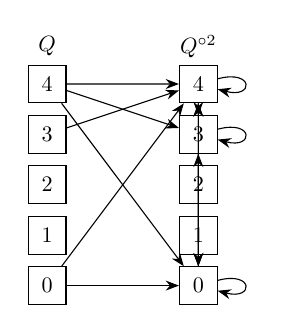
\begin{tikzpicture}[>=Stealth,scale=0.8,every node/.append style={transform shape}]
  \radcol{0}{$Q$}{L}
  \radcol{2.4}{$Q^{\circ2}$}{M}
  \draw[->] (L0) -- (M0); \draw[->] (L0) -- (M4); \draw[->] (L3) -- (M4); \draw[->] (L4) -- (M0); \draw[->] (L4) -- (M3); \draw[->] (L4) -- (M4);
  \draw[->] (M0) edge[loop right,min distance=6mm] (M0); \draw[->] (M0) -- (M3); \draw[->] (M0) -- (M4); \draw[->] (M3) -- (M0); \draw[->] (M3) edge[loop right,min distance=6mm] (M3); \draw[->] (M3) -- (M4);
  \draw[->] (M4) -- (M0); \draw[->] (M4) -- (M3); \draw[->] (M4) edge[loop right,min distance=6mm] (M4);
\end{tikzpicture}
\end{center}
\centerline{$AD(Q^{\circ2}\circ Q)$}
Chasing from $0$, $3$, $4$ each lands on $\{0,3,4\}$ again --- identical to $Q^{\circ2}$.
\[
Q^{\circ3} = \{(0,0),(0,3),(0,4),(3,0),(3,3),(3,4),(4,0),(4,3),(4,4)\} = Q^{\circ2}
\]
Stabilized: $Q^{\circ4}=Q^{\circ5}=Q^{\circ2}$, by the same repeat-once-stable argument as part (vii).

\seclabel{1abc.ix.6}
\[
Q^{\circ4}=Q^{\circ2}=\{(0,0),(0,3),(0,4),(3,0),(3,3),(3,4),(4,0),(4,3),(4,4)\}, \qquad Q^{\circ5}=Q^{\circ2}
\]

\seclabel{1abc.ix.7}
\noindent\textbf{Why stopping at $k=5$ is enough (pigeonhole), including $k=0$ for reflexivity:} $\nu(\{0,..,4\})=5$; any path needing more than $5$ edges has a shorter equivalent (delete the revisited-vertex cycle), so checking $Q^{\circ0}$ through $Q^{\circ5}$ catches every pair. Note $Q$ never relates vertex $1$ or $2$ to anything, so $(1,1)$ and $(2,2)$ enter only through $Q^{\circ0}:=\Delta$.
\[
\bigcup_{k=0}^{5}\big((R\cup(R^{op}))^{\circ k}\big) = Q^{\circ0}\cup Q^{\circ1}\cup Q^{\circ2}\cup Q^{\circ3}\cup Q^{\circ4}\cup Q^{\circ5}
\]
\[
= \{(0,0),(1,1),(2,2),(3,3),(4,4)\}\cup\{(0,0),(0,4),(3,4),(4,0),(4,3),(4,4)\}
\]
\[
\cup\{(0,0),(0,3),(0,4),(3,0),(3,3),(3,4),(4,0),(4,3),(4,4)\}
\]
\[
= \{(0,0),(0,3),(0,4),(1,1),(2,2),(3,0),(3,3),(3,4),(4,0),(4,3),(4,4)\}
\]

\seclabel{1abc.ix.8}
$\big(M(\bigcup_{k=0}^5(R\cup(R^{op}))^{\circ k})\big)(0,1)$:
\begin{center}
\begin{tabular}{c|ccccc}
& 0&1&2&3&4\\\hline
0 & 1&0&0&1&1\\
1 & 0&1&0&0&0\\
2 & 0&0&1&0&0\\
3 & 1&0&0&1&1\\
4 & 1&0&0&1&1
\end{tabular}
\qquad
$=\begin{bmatrix}1&0&0&1&1\\0&1&0&0&0\\0&0&1&0&0\\1&0&0&1&1\\1&0&0&1&1\end{bmatrix}$
\end{center}

\noindent\textbf{Prove:} $\big(M(\EqvClsr(R))\big)(0,1) = \big(M(\bigcup_{k=0}^5(R\cup(R^{op}))^{\circ k})\big)(0,1)$.
\[
\text{LS}=\begin{bmatrix}1&0&0&1&1\\0&1&0&0&0\\0&0&1&0&0\\1&0&0&1&1\\1&0&0&1&1\end{bmatrix}=\text{RS}
\]
\centerline{LS $=$ RS}

\clearpage
\section*{2a --- injective/surjective functions $A\to B$}
$A=\{0,1,10\}$, $\nu(A)=3$. $\quad B=\{0,1,4,9\}$, $\nu(B)=4$. Four \emph{separate} propositions, one function-name each ($\alpha,\beta,\gamma,\delta$), with the injective/surjective conjunct struck through wherever it's \emph{negated}:
\[
\text{(i) }\exists\alpha\big((\Inj(\alpha))\wedge(\Srj(\alpha))\big),\quad
\text{(ii) }\exists\beta\big((\text{\sout{\textit{Inj}}}(\beta))\wedge(\Srj(\beta))\big),
\]
\[
\text{(iii) }\exists\gamma\big((\Inj(\gamma))\wedge(\text{\sout{\textit{Srj}}}(\gamma))\big),\quad
\text{(iv) }\exists\delta\big((\text{\sout{\textit{Inj}}}(\delta))\wedge(\text{\sout{\textit{Srj}}}(\delta))\big)
\]

\seclabel{2a.0}
\noindent\textbf{Lemmas used below} (standard facts about finite functions):
\[
\begin{array}{c}
\InjFncs(A,B)\ne\{\}\\
\hline\hline
\nu(A)\le\nu(B)
\end{array}
\qquad\qquad\qquad
\begin{array}{c}
\SrjFncs(A,B)\ne\{\}\\
\hline\hline
\nu(A)\ge\nu(B)
\end{array}
\]
Here $\nu(A)=3<4=\nu(B)$, so the right-hand lemma immediately gives $\SrjFncs(A,B)=\{\}$: \textbf{no} function $A\to B$ is ever surjective, full stop. That one fact drives (i)--(iv) below.

\subsection*{(i) \circn\ --- impossible}
\seclabel{2a.i}
\[
\begin{array}{cc}
\alpha\in\Fnc(A,B) & I:=\Img(\alpha)\\
\Inj(\alpha)\wedge\Srj(\alpha) & \nu(A)=3,\ \nu(B)=4\\
\hline
\multicolumn{2}{c}{\Srj(\alpha)}\\
\hline
\multicolumn{2}{c}{\nu(I)=\nu(B)=4}\\
\hline
\multicolumn{2}{c}{\nu(I)\le\nu(A)=3}\\
\hline
\multicolumn{2}{c}{4\le3}\\
\hline
\multicolumn{2}{c}{\bot}\\
\hline
\multicolumn{2}{c}{\neg\exists\alpha\in\Fnc(A,B)\big((\Inj(\alpha))\wedge(\Srj(\alpha))\big)}
\end{array}
\]

\subsection*{(ii) \circn\ --- impossible}
\seclabel{2a.ii}
\[
\begin{array}{cc}
\beta\in\Fnc(A,B) & I:=\Img(\beta)\\
\Srj(\beta) & \nu(A)=3,\ \nu(B)=4\\
\hline
\multicolumn{2}{c}{\nu(I)=\nu(B)=4}\\
\hline
\multicolumn{2}{c}{\nu(I)\le\nu(A)=3}\\
\hline
\multicolumn{2}{c}{4\le3}\\
\hline
\multicolumn{2}{c}{\bot}\\
\hline
\multicolumn{2}{c}{\neg\exists\beta\in\Fnc(A,B)\big((\text{\sout{\textit{Inj}}}(\beta))\wedge(\Srj(\beta))\big)}
\end{array}
\]

\subsection*{(iii) \circy\ --- witnessed}
\seclabel{2a.iii}
Since $\nu(A)=3\le4=\nu(B)$, the lemma gives $\InjFncs(A,B)\ne\{\}$, so injective functions $A\to B$ exist; and \emph{every} function $A\to B$ automatically satisfies $\neg\Srj$ (shown above), so any injective witness works. Take
\[
\gamma:A\to B,\qquad \gamma(0)=0,\quad \gamma(1)=1,\quad \gamma(10)=4
\]
\begin{center}
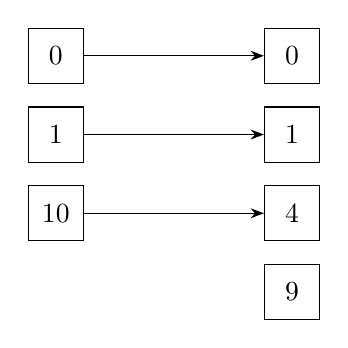
\begin{tikzpicture}[scale=1,>=Stealth]
  \node[draw,rectangle,minimum size=7mm] (a0) at (0,2) {0};
  \node[draw,rectangle,minimum size=7mm] (a1) at (0,1) {1};
  \node[draw,rectangle,minimum size=7mm] (a2) at (0,0) {10};
  \node[draw,rectangle,minimum size=7mm] (b0) at (3,2) {0};
  \node[draw,rectangle,minimum size=7mm] (b1) at (3,1) {1};
  \node[draw,rectangle,minimum size=7mm] (b2) at (3,0) {4};
  \node[draw,rectangle,minimum size=7mm] (b3) at (3,-1) {9};
  \draw[->] (a0) -- (b0);
  \draw[->] (a1) -- (b1);
  \draw[->] (a2) -- (b2);
\end{tikzpicture}
\end{center}
$\Img(\gamma)=\{0,1,4\}$, all three outputs distinct $\Rightarrow \Inj(\gamma)$. $9\notin\Img(\gamma) \Rightarrow \neg\Srj(\gamma)$. So $\Inj(\gamma)\wedge\neg\Srj(\gamma)$ holds:
\[
\therefore \exists\gamma\in\Fnc(A,B)\big((\Inj(\gamma))\wedge(\text{\sout{\textit{Srj}}}(\gamma))\big) \qquad\checkmark
\]

\subsection*{(iv) \circy\ --- witnessed}
\seclabel{2a.iv}
Every function $A\to B$ is automatically $\neg\Srj$ (shown above), so we only need \emph{some} non-injective $\delta$. Take
\[
\delta:A\to B,\qquad \delta(0)=0,\quad \delta(1)=1,\quad \delta(10)=1
\]
\begin{center}
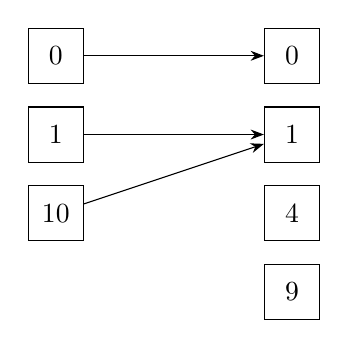
\begin{tikzpicture}[scale=1,>=Stealth]
  \node[draw,rectangle,minimum size=7mm] (a0) at (0,2) {0};
  \node[draw,rectangle,minimum size=7mm] (a1) at (0,1) {1};
  \node[draw,rectangle,minimum size=7mm] (a2) at (0,0) {10};
  \node[draw,rectangle,minimum size=7mm] (b0) at (3,2) {0};
  \node[draw,rectangle,minimum size=7mm] (b1) at (3,1) {1};
  \node[draw,rectangle,minimum size=7mm] (b2) at (3,0) {4};
  \node[draw,rectangle,minimum size=7mm] (b3) at (3,-1) {9};
  \draw[->] (a0) -- (b0);
  \draw[->] (a1) -- (b1);
  \draw[->] (a2) -- (b1);
\end{tikzpicture}
\end{center}
$\delta(1)=\delta(10)=1$ with $1\ne10 \Rightarrow \neg\Inj(\delta)$. $\Img(\delta)=\{0,1\}\ne B \Rightarrow \neg\Srj(\delta)$. So $\neg\Inj(\delta)\wedge\neg\Srj(\delta)$ holds:
\[
\therefore \exists\delta\in\Fnc(A,B)\big((\text{\sout{\textit{Inj}}}(\delta))\wedge(\text{\sout{\textit{Srj}}}(\delta))\big) \qquad\checkmark
\]

\subsection*{(v)--(vi): image and maximal bijective restrictions of $\delta$}
\seclabel{2a.v-vi}
\[
\Img(\delta) = \{0,1\}
\]
Since $\delta(1)=\delta(10)=1$, any subset of $A$ containing \emph{both} $1$ and $10$ fails injectivity. The maximal subsets of $A$ on which $\delta$ is injective are $\{0,1\}$ and $\{0,10\}$:
\begin{center}
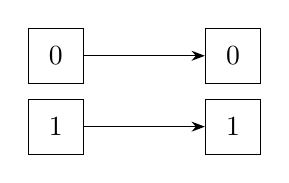
\begin{tikzpicture}[scale=0.9,>=Stealth]
  \node[draw,rectangle,minimum size=7mm] (a0) at (0,1.5) {0};
  \node[draw,rectangle,minimum size=7mm] (a1) at (0,0.5) {1};
  \node[draw,rectangle,minimum size=7mm] (b0) at (2.5,1.5) {0};
  \node[draw,rectangle,minimum size=7mm] (b1) at (2.5,0.5) {1};
  \draw[->] (a0)--(b0); \draw[->] (a1)--(b1);
\end{tikzpicture}
\hspace{1.5cm}
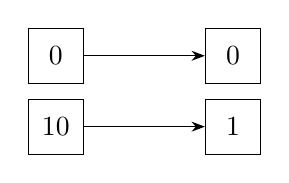
\begin{tikzpicture}[scale=0.9,>=Stealth]
  \node[draw,rectangle,minimum size=7mm] (a0) at (0,1.5) {0};
  \node[draw,rectangle,minimum size=7mm] (a2) at (0,0.5) {10};
  \node[draw,rectangle,minimum size=7mm] (b0) at (2.5,1.5) {0};
  \node[draw,rectangle,minimum size=7mm] (b1) at (2.5,0.5) {1};
  \draw[->] (a0)--(b0); \draw[->] (a2)--(b1);
\end{tikzpicture}
\end{center}
\centerline{$\delta|_{\{0,1\}}:\{0,1\}\to\{0,1\}$ \hspace{2.5cm} $\delta|_{\{0,10\}}:\{0,10\}\to\{0,1\}$}
Both restrictions are bijections onto $\{0,1\}$. Count of maximal injective (adjusted-bijective) restrictions $=\mathbf{2}$.

\clearpage
\section*{2b --- $R$ (same parity) and $S$ (order-or-divides)}
$R:=\{(j,k)\in J\times J\mid 2\mid|j-k|\}$, $J=\{0,1,3,4,7,9\}$.

\subsection*{(i) \circy\ $\Eqv(R)$}
\seclabel{2b.i}
Exhaustive check of all $36$ pairs of $J\times J$ (condition on top, membership conclusion below):
\begingroup\tiny\setlength{\arraycolsep}{2pt}
\[
\begin{array}{cccccc}
\dfrac{Evn(0+0)}{(0,0)\in R} & \dfrac{Evn(|0-1|)}{(0,1)\notin R} & \dfrac{Evn(|0-3|)}{(0,3)\notin R} & \dfrac{Evn(|0-4|)}{(0,4)\in R} & \dfrac{Evn(|0-7|)}{(0,7)\notin R} & \dfrac{Evn(|0-9|)}{(0,9)\notin R} \\[3mm]
\dfrac{Evn(|1-0|)}{(1,0)\notin R} & \dfrac{Evn(1+1)}{(1,1)\in R} & \dfrac{Evn(|1-3|)}{(1,3)\in R} & \dfrac{Evn(|1-4|)}{(1,4)\notin R} & \dfrac{Evn(|1-7|)}{(1,7)\in R} & \dfrac{Evn(|1-9|)}{(1,9)\in R} \\[3mm]
\dfrac{Evn(|3-0|)}{(3,0)\notin R} & \dfrac{Evn(|3-1|)}{(3,1)\in R} & \dfrac{Evn(3+3)}{(3,3)\in R} & \dfrac{Evn(|3-4|)}{(3,4)\notin R} & \dfrac{Evn(|3-7|)}{(3,7)\in R} & \dfrac{Evn(|3-9|)}{(3,9)\in R} \\[3mm]
\dfrac{Evn(|4-0|)}{(4,0)\in R} & \dfrac{Evn(|4-1|)}{(4,1)\notin R} & \dfrac{Evn(|4-3|)}{(4,3)\notin R} & \dfrac{Evn(4+4)}{(4,4)\in R} & \dfrac{Evn(|4-7|)}{(4,7)\notin R} & \dfrac{Evn(|4-9|)}{(4,9)\notin R} \\[3mm]
\dfrac{Evn(|7-0|)}{(7,0)\notin R} & \dfrac{Evn(|7-1|)}{(7,1)\in R} & \dfrac{Evn(|7-3|)}{(7,3)\in R} & \dfrac{Evn(|7-4|)}{(7,4)\notin R} & \dfrac{Evn(7+7)}{(7,7)\in R} & \dfrac{Evn(|7-9|)}{(7,9)\in R} \\[3mm]
\dfrac{Evn(|9-0|)}{(9,0)\notin R} & \dfrac{Evn(|9-1|)}{(9,1)\in R} & \dfrac{Evn(|9-3|)}{(9,3)\in R} & \dfrac{Evn(|9-4|)}{(9,4)\notin R} & \dfrac{Evn(|9-7|)}{(9,7)\in R} & \dfrac{Evn(9+9)}{(9,9)\in R}
\end{array}
\]
\endgroup
\begin{center}\small
$R = \{(0,0),(0,4),(1,1),(1,3),(1,7),(1,9),(3,1),(3,3),(3,7),(3,9),$\\
$(4,0),(4,4),(7,1),(7,3),(7,7),(7,9),(9,1),(9,3),(9,7),(9,9)\}$
\end{center}
Splits $J$ by parity: evens $\{0,4\}$, odds $\{1,3,7,9\}$.
\[
\begin{array}{ll}
j\in J \Rightarrow |j-j|=0,\ 2\mid0 \Rightarrow (j,j)\in R & \op{Rflx}(R)\\
(j,k)\in R \Rightarrow 2\mid|j-k| = |k-j| \Rightarrow (k,j)\in R & \op{Sym}(R)\\
(j,k),(k,l)\in R \Rightarrow j,k\text{ same parity},\ k,l\text{ same parity} \Rightarrow j,l\text{ same parity} \Rightarrow (j,l)\in R & \op{Trns}(R)
\end{array}
\]
\[
\op{Rflx}(R)\wedge\op{Sym}(R)\wedge\op{Trns}(R)\ \Rightarrow\ \Eqv(R)
\]
\begin{center}
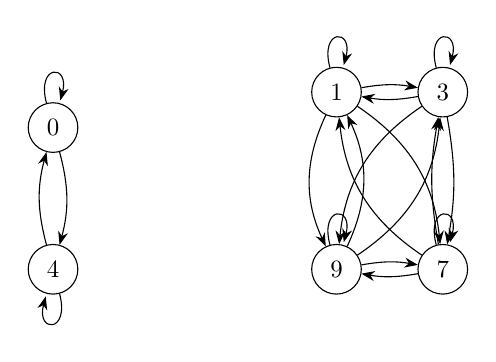
\begin{tikzpicture}[every node/.style={draw,circle,minimum size=7mm},>=Stealth,scale=0.9,every node/.append style={transform shape}]
  \node (a) at (0,1) {0}; \node (b) at (0,-1) {4};
  \draw[->] (a) edge [loop above] (a); \draw[->] (b) edge [loop below] (b);
  \draw[->] (a) edge[bend left=15] (b); \draw[->] (b) edge[bend left=15] (a);
  \node (c) at (4,1.5) {1}; \node (d) at (5.5,1.5) {3}; \node (e) at (5.5,-1) {7}; \node (f) at (4,-1) {9};
  \foreach \n in {c,d,e,f} \draw[->] (\n) edge [loop above] (\n);
  \draw[->] (c) edge[bend left=10] (d); \draw[->] (d) edge[bend left=10] (c);
  \draw[->] (d) edge[bend left=10] (e); \draw[->] (e) edge[bend left=10] (d);
  \draw[->] (e) edge[bend left=10] (f); \draw[->] (f) edge[bend left=10] (e);
  \draw[->] (c) edge[bend left=25] (e); \draw[->] (e) edge[bend left=25] (c);
  \draw[->] (c) edge[bend right=25] (f); \draw[->] (f) edge[bend right=25] (c);
  \draw[->] (d) edge[bend right=25] (f); \draw[->] (f) edge[bend right=25] (d);
\end{tikzpicture}
\end{center}
Two complete cliques (with self-loops) --- one on $\{0,4\}$, one on $\{1,3,7,9\}$ --- and \emph{no} edges between them. Classes: $\{0,4\}$, $\{1,3,7,9\}$.

\subsection*{(ii) \circn\ $\PO(S)$}
\seclabel{2b.ii}
$S:=\{(e,f)\in E\times E\mid(e\ge f)\vee(e\mid f)\}$, $E=\{0,1,4,9\}$. Exhaustive check of all $16$ pairs of $E\times E$:
\begingroup\scriptsize
\[
\begin{array}{cccc}
\dfrac{(0\ge0)\vee(0\mid0)}{(0,0)\in S} & \dfrac{(0\ge1)\vee(0\mid1)}{(0,1)\notin S} & \dfrac{(0\ge4)\vee(0\mid4)}{(0,4)\notin S} & \dfrac{(0\ge9)\vee(0\mid9)}{(0,9)\notin S} \\[3mm]
\dfrac{(1\ge0)\vee(1\mid0)}{(1,0)\in S} & \dfrac{(1\ge1)\vee(1\mid1)}{(1,1)\in S} & \dfrac{(1\ge4)\vee(1\mid4)}{(1,4)\in S} & \dfrac{(1\ge9)\vee(1\mid9)}{(1,9)\in S} \\[3mm]
\dfrac{(4\ge0)\vee(4\mid0)}{(4,0)\in S} & \dfrac{(4\ge1)\vee(4\mid1)}{(4,1)\in S} & \dfrac{(4\ge4)\vee(4\mid4)}{(4,4)\in S} & \dfrac{(4\ge9)\vee(4\mid9)}{(4,9)\notin S} \\[3mm]
\dfrac{(9\ge0)\vee(9\mid0)}{(9,0)\in S} & \dfrac{(9\ge1)\vee(9\mid1)}{(9,1)\in S} & \dfrac{(9\ge4)\vee(9\mid4)}{(9,4)\in S} & \dfrac{(9\ge9)\vee(9\mid9)}{(9,9)\in S}
\end{array}
\]
\endgroup
\[
S = \{(0,0),(1,0),(1,1),(1,4),(1,9),(4,0),(4,1),(4,4),(9,0),(9,1),(9,4),(9,9)\}
\]
\[
\begin{array}{c}
1,4\in E,\quad 1\mid4\ \text{(long division: }4=1\times4+0\text{)},\quad 4\ge1\\
\hline
(1,4)\in S \qquad (4,1)\in S \qquad 1\ne4\\
\hline
\neg\op{AntSym}(S)\\
\hline
\neg\PO(S)
\end{array}
\]

\clearpage
\section*{2c --- $R(\varphi):=\{(u,v)\mid \varphi(u)=\varphi(v)\}$, given $\PO(T,\le)$}
\seclabel{2c}
Claim: $\forall\varphi\in\Fnc(S,T)\ \PO(R(\varphi))$. \circn.

\noindent\textbf{Rflx and Sym always hold, for any $\varphi$} (needed before the counterexample below):
\[
\begin{array}{c}
u\in S,\quad \varphi(u)=\varphi(u)\\
\hline
(u,u)\in R(\varphi)\\
\hline
\op{Rflx}(R(\varphi))
\end{array}
\qquad\qquad
\begin{array}{c}
(u,v)\in R(\varphi),\quad \varphi(u)=\varphi(v)\\
\hline
\varphi(v)=\varphi(u)\\
\hline
(v,u)\in R(\varphi)\\
\hline
\op{Sym}(R(\varphi))
\end{array}
\]
\noindent\textbf{Counterexample:} take $\varphi$ \emph{constant}, $\varphi(x):=0$ for all $x\in S$ (valid since $T\ne\{\}$; label the constant value $0$). Since $\nu(S)\ge2$, let $0,1$ denote two distinct elements of $S$ (relabeling if necessary):
\begin{center}
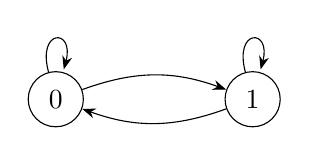
\begin{tikzpicture}[every node/.style={draw,circle,minimum size=7mm},>=Stealth,scale=1]
  \node (u) at (0,0) {$0$}; \node (v) at (2.5,0) {$1$};
  \draw[->] (u) edge [loop above] (u); \draw[->] (v) edge [loop above] (v);
  \draw[->] (u) edge[bend left=20] (v); \draw[->] (v) edge[bend left=20] (u);
\end{tikzpicture}
\end{center}
\[
\begin{array}{c}
\varphi(0)=0=\varphi(1)\\
\hline
(0,1)\in R(\varphi) \qquad (1,0)\in R(\varphi) \qquad 0\ne1\\
\hline
\neg\op{AntSym}(R(\varphi))\\
\hline
\neg\PO(R(\varphi))\\
\hline
\neg\big(\forall\varphi\in\Fnc(S,T)\ \PO(R(\varphi))\big)
\end{array}
\]

\clearpage
\section*{3a --- $P$ and $Q$ (divisibility orders)}
$J=\{0,1,3,4,7,9\}$, $\quad E=\{0,1,4,9\}$.

\subsection*{(i) \circy\ $\PO(P)$, $P:=\{(j,k)\in J\times J\mid j\mid k\}$}
\seclabel{3a.i}
Exhaustive check of all $36$ pairs of $J\times J$:
\begingroup\tiny\setlength{\arraycolsep}{2pt}
\[
\begin{array}{cccccc}
\dfrac{0\mid0}{(0,0)\in P} & \dfrac{0\nmid1}{(0,1)\notin P} & \dfrac{0\nmid3}{(0,3)\notin P} & \dfrac{0\nmid4}{(0,4)\notin P} & \dfrac{0\nmid7}{(0,7)\notin P} & \dfrac{0\nmid9}{(0,9)\notin P} \\[3mm]
\dfrac{1\mid0}{(1,0)\in P} & \dfrac{1\mid1}{(1,1)\in P} & \dfrac{1\mid3}{(1,3)\in P} & \dfrac{1\mid4}{(1,4)\in P} & \dfrac{1\mid7}{(1,7)\in P} & \dfrac{1\mid9}{(1,9)\in P} \\[3mm]
\dfrac{3\mid0}{(3,0)\in P} & \dfrac{3\nmid1}{(3,1)\notin P} & \dfrac{3\mid3}{(3,3)\in P} & \dfrac{3\nmid4}{(3,4)\notin P} & \dfrac{3\nmid7}{(3,7)\notin P} & \dfrac{3\mid9}{(3,9)\in P} \\[3mm]
\dfrac{4\mid0}{(4,0)\in P} & \dfrac{4\nmid1}{(4,1)\notin P} & \dfrac{4\nmid3}{(4,3)\notin P} & \dfrac{4\mid4}{(4,4)\in P} & \dfrac{4\nmid7}{(4,7)\notin P} & \dfrac{4\nmid9}{(4,9)\notin P} \\[3mm]
\dfrac{7\mid0}{(7,0)\in P} & \dfrac{7\nmid1}{(7,1)\notin P} & \dfrac{7\nmid3}{(7,3)\notin P} & \dfrac{7\nmid4}{(7,4)\notin P} & \dfrac{7\mid7}{(7,7)\in P} & \dfrac{7\nmid9}{(7,9)\notin P} \\[3mm]
\dfrac{9\mid0}{(9,0)\in P} & \dfrac{9\nmid1}{(9,1)\notin P} & \dfrac{9\nmid3}{(9,3)\notin P} & \dfrac{9\nmid4}{(9,4)\notin P} & \dfrac{9\nmid7}{(9,7)\notin P} & \dfrac{9\mid9}{(9,9)\in P}
\end{array}
\]
\endgroup
\begin{center}\small
$P = \{(0,0),(1,0),(1,1),(1,3),(1,4),(1,7),(1,9),(3,0),$\\
$(3,3),(3,9),(4,0),(4,4),(7,0),(7,7),(9,0),(9,9)\}$
\end{center}
\[
\op{Rflx}: j=j\times1\Rightarrow j\mid j\qquad
\op{AntSym}: j\mid k \wedge k\mid j \Rightarrow j=k\qquad
\op{Trns}: j\mid k\wedge k\mid l \Rightarrow j\mid l
\]
Cover relation, verified by division ($a\mid b$ iff $b\div a$ has remainder $0$):
\[
1\mid3\,(3{=}1{\times}3{+}0),\quad1\mid4\,(4{=}1{\times}4{+}0),\quad1\mid7\,(7{=}1{\times}7{+}0),\quad3\mid9\,(9{=}3{\times}3{+}0)
\]
\[
4\mid0,\quad7\mid0,\quad9\mid0\qquad(\text{every }j\text{ divides }0\text{ since }0=j\times0+0)
\]
\begin{center}
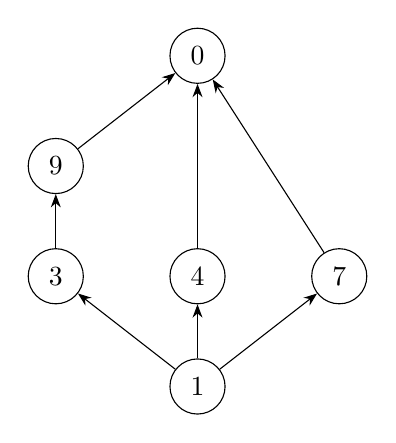
\begin{tikzpicture}[every node/.style={draw,circle,minimum size=7mm,inner sep=1pt},>=Stealth,scale=1,every node/.append style={transform shape}]
  \node (h1) at (0,0) {1}; \node (h3) at (-1.8,1.4) {3}; \node (h4) at (0,1.4) {4};
  \node (h7) at (1.8,1.4) {7}; \node (h9) at (-1.8,2.8) {9}; \node (h0) at (0,4.2) {0};
  \draw[->] (h1)--(h3); \draw[->] (h1)--(h4); \draw[->] (h1)--(h7); \draw[->] (h3)--(h9);
  \draw[->] (h4)--(h0); \draw[->] (h7)--(h0); \draw[->] (h9)--(h0);
\end{tikzpicture}
\end{center}
Bottom $1$, covered by $3,4,7$; $9$ covers $3$; top $0$ covers $4,7,9$. Arrows point from the covered (smaller) element up to the covering (larger) element, per $HsDgrm$ convention. (Note: $1\lessdot9$ is \emph{not} a direct cover --- $1\mid3\mid9$ gives a longer path, so the edge $1$--$9$ is not drawn.)

\subsection*{(ii) \circy\ $\PO(Q)$, $Q:=\{(e,f)\in E\times E\mid f\mid e\}$}
\seclabel{3a.ii}
Exhaustive check of all $16$ pairs of $E\times E$ (test label shows $f\mid e$, concluding membership of pair $(e,f)$):
\begingroup\scriptsize
\[
\begin{array}{cccc}
\dfrac{0\mid0}{(0,0)\in Q} & \dfrac{1\mid0}{(0,1)\in Q} & \dfrac{4\mid0}{(0,4)\in Q} & \dfrac{9\mid0}{(0,9)\in Q} \\[3mm]
\dfrac{0\nmid1}{(1,0)\notin Q} & \dfrac{1\mid1}{(1,1)\in Q} & \dfrac{4\nmid1}{(1,4)\notin Q} & \dfrac{9\nmid1}{(1,9)\notin Q} \\[3mm]
\dfrac{0\nmid4}{(4,0)\notin Q} & \dfrac{1\mid4}{(4,1)\in Q} & \dfrac{4\mid4}{(4,4)\in Q} & \dfrac{9\nmid4}{(4,9)\notin Q} \\[3mm]
\dfrac{0\nmid9}{(9,0)\notin Q} & \dfrac{1\mid9}{(9,1)\in Q} & \dfrac{4\nmid9}{(9,4)\notin Q} & \dfrac{9\mid9}{(9,9)\in Q}
\end{array}
\]
\endgroup
\[
Q = \{(0,0),(0,1),(0,4),(0,9),(1,1),(4,1),(4,4),(9,1),(9,9)\}
\]
Same three steps, with the divisibility direction flipped ($f\mid e$ instead of $e\mid f$):
\[
\op{Rflx}(Q)\quad\op{AntSym}(Q)\quad\op{Trns}(Q)\ \Rightarrow\ \PO(Q)
\]
Cover relation: an edge $(x,y)$ of $Q$ (meaning $x\le y$) requires $y\mid x$. Checking all pairs of $E=\{0,1,4,9\}$:
\[
4\mid0\,(0{=}4{\times}0{+}0)\Rightarrow0\le4,\qquad 9\mid0\,(0{=}9{\times}0{+}0)\Rightarrow0\le9
\]
\[
1\mid4\,(4{=}1{\times}4{+}0)\Rightarrow4\le1,\qquad 1\mid9\,(9{=}1{\times}9{+}0)\Rightarrow9\le1
\]
\begin{center}
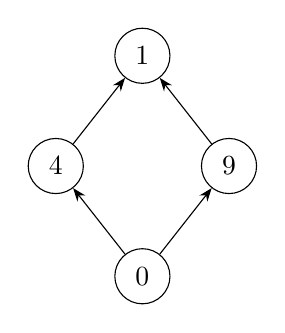
\begin{tikzpicture}[every node/.style={draw,circle,minimum size=7mm,inner sep=1pt},>=Stealth,scale=1,every node/.append style={transform shape}]
  \node (h0) at (0,0) {0}; \node (h4) at (-1.1,1.4) {4}; \node (h9) at (1.1,1.4) {9}; \node (h1) at (0,2.8) {1};
  \draw[->] (h0)--(h4); \draw[->] (h0)--(h9); \draw[->] (h4)--(h1); \draw[->] (h9)--(h1);
\end{tikzpicture}
\end{center}
Bottom $0$, covered by $4,9$; top $1$ covers $4,9$. Arrows point from covered to covering element.
\emph{(Since $E$ has no element like $3$ between $1$ and $4$ or $9$ under this order, both $0$--$4$--$1$ and $0$--$9$--$1$ are genuine direct covers, unlike part (i). Double-check against the pairwise table above: $Q$ places $0$ at the bottom and $1$ at the top, since $(0,1)\in Q$ but $(1,0)\notin Q$ --- a solved-exam sample that draws this Hasse diagram with $0$ at the top has it backwards.)}

\clearpage
\section*{3b --- symmetric-difference of equivalence relations}
Given a set $S$ and $E,F\in\EqvRlns(S,S)$.

\subsection*{(i) \circn\ $\Eqv(E\setminus F)$}
\seclabel{3b.i}
\[
\begin{array}{c}
F\in\EqvRlns(S,S)\\
\hline
\op{Rflx}(F)\\
\hline
\Delta_S\subseteq F\\
\hline
\forall x\in S,\ (x,x)\in F\\
\hline
\forall x\in S,\ (x,x)\notin E\setminus F\\
\hline
\neg\op{Rflx}(E\setminus F)\\
\hline
\neg\Eqv(E\setminus F)
\end{array}
\]

\subsection*{(ii) \circn\ $\Eqv\big((E\setminus F)\cup(F\setminus E)\big)$}
\seclabel{3b.ii}
\[
\begin{array}{c}
E,F\in\EqvRlns(S,S)\\
\hline
\Delta_S\subseteq E \qquad \Delta_S\subseteq F\\
\hline
\Delta_S\subseteq(E\cap F)\\
\hline
\forall x\in S,\ (x,x)\in E\cap F\\
\hline
\forall x\in S,\ (x,x)\notin(E\setminus F)\cup(F\setminus E)\\
\hline
\neg\op{Rflx}\big((E\setminus F)\cup(F\setminus E)\big)\\
\hline
\neg\Eqv\big((E\setminus F)\cup(F\setminus E)\big)
\end{array}
\]

\begin{center}
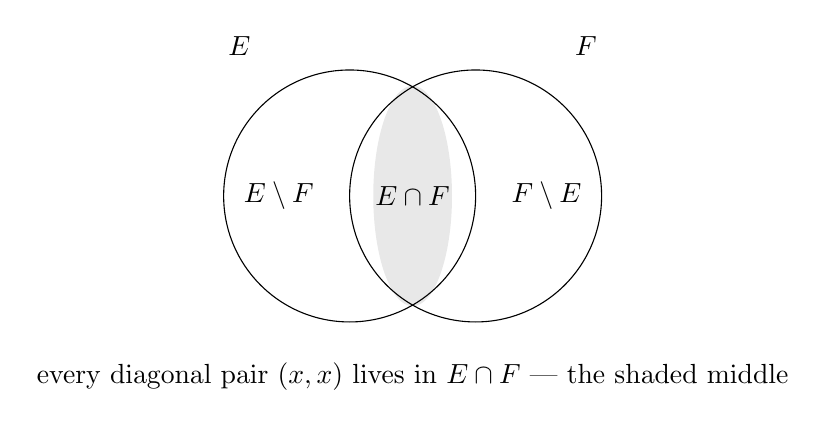
\begin{tikzpicture}[scale=1]
  \fill[gray!30,opacity=0.6] (0.8,0) ellipse (0.5cm and 1.4cm);
  \draw (0,0) circle (1.6cm);
  \draw (1.6,0) circle (1.6cm);
  \node at (-1.4,1.9) {$E$};
  \node at (3.0,1.9) {$F$};
  \node at (-0.9,0) {$E\setminus F$};
  \node at (2.5,0) {$F\setminus E$};
  \node at (0.8,0) {$E\cap F$};
  \node[align=center] at (0.8,-2.3) {every diagonal pair $(x,x)$ lives in $E\cap F$ --- the shaded middle};
\end{tikzpicture}
\end{center}
The diagonal $\Delta_S$ always sits in the overlap $E\cap F$ (both are reflexive), so it can never appear in $E\setminus F$, $F\setminus E$, or their union --- reflexivity fails every time, for every $S,E,F$.

\clearpage
\section*{3c --- counting on $B=\{0,1,4,9\}$, $\nu(B)=4$}
\seclabel{3c}

\subsection*{$\nu(\op{TtlOrdrs}(B)) = 4! = 24$ --- long multiplication}
\[
4! = 4\times3\times2\times1
\]
\[
4\times3 = 12,\qquad 12\times2 = 24,\qquad 24\times1 = 24
\]
$\op{TtlOrdrs}(B)$: all $24$ permutations of $\{0,1,4,9\}$ read as chains:
\begin{center}
\begin{tabular}{llll}
$0{<}1{<}4{<}9$ & $0{<}1{<}9{<}4$ & $0{<}4{<}1{<}9$ & $0{<}4{<}9{<}1$\\
$0{<}9{<}1{<}4$ & $0{<}9{<}4{<}1$ & $1{<}0{<}4{<}9$ & $1{<}0{<}9{<}4$\\
$1{<}4{<}0{<}9$ & $1{<}4{<}9{<}0$ & $1{<}9{<}0{<}4$ & $1{<}9{<}4{<}0$\\
$4{<}0{<}1{<}9$ & $4{<}0{<}9{<}1$ & $4{<}1{<}0{<}9$ & $4{<}1{<}9{<}0$\\
$4{<}9{<}0{<}1$ & $4{<}9{<}1{<}0$ & $9{<}0{<}1{<}4$ & $9{<}0{<}4{<}1$\\
$9{<}1{<}0{<}4$ & $9{<}1{<}4{<}0$ & $9{<}4{<}0{<}1$ & $9{<}4{<}1{<}0$
\end{tabular}
\end{center}

\subsection*{$\nu(\EqvRlns(B))=\nu(\Prtns(B)) = B_4 = 15$ --- via Stirling numbers of the 2nd kind}
$B_4 = \sum_{k=0}^{4} S(4,k)$, where $S(n,k)$ = number of ways to split $n$ labeled elements into exactly $k$ nonempty unlabeled groups, via the recurrence $S(n,k)=k\!\cdot\! S(n-1,k)+S(n-1,k-1)$, base $S(0,0)=1$, $S(n,0)=S(0,k)=0$ otherwise.

\[
\begin{array}{|c|ccccc|}
\hline
n\backslash k & 0 & 1 & 2 & 3 & 4\\\hline
0 & 1 & 0 & 0 & 0 & 0\\
1 & 0 & 1 & 0 & 0 & 0\\
2 & 0 & 1 & 1 & 0 & 0\\
3 & 0 & 1 & 3 & 1 & 0\\
4 & 0 & 1 & 7 & 6 & 1\\\hline
\end{array}
\]
Sample recurrence steps: $S(3,2)=2\cdot S(2,2)+S(2,1)=2(1)+1=3$. $\ S(4,2)=2\cdot S(3,2)+S(3,1)=2(3)+1=7$. $\ S(4,3)=3\cdot S(3,3)+S(3,2)=3(1)+3=6$.
\[
B_4 = S(4,0)+S(4,1)+S(4,2)+S(4,3)+S(4,4) = 0+1+7+6+1 = 15
\]
$\Prtns(B)$, all $15$ (grouped by shape --- $S(4,1)=1$ way to make one group of 4, $S(4,2)=7$ ways to split into two groups, $S(4,3)=6$ ways into three groups, $S(4,4)=1$ way into four singletons):
\begin{center}
\begin{tabular}{l}
\{0,1,4,9\} \hfill\textit{(1 way, all together)}\\[2mm]
\{0\},\{1,4,9\}\quad \{1\},\{0,4,9\}\quad \{4\},\{0,1,9\}\quad \{9\},\{0,1,4\}\hfill\textit{(4 of the 7 two-group ways: one singleton)}\\
\{0,1\},\{4,9\}\quad \{0,4\},\{1,9\}\quad \{0,9\},\{1,4\}\hfill\textit{(remaining 3 of the 7: two pairs)}\\[2mm]
\{0\},\{1\},\{4,9\}\quad \{0\},\{4\},\{1,9\}\quad \{0\},\{9\},\{1,4\}\quad \{1\},\{4\},\{0,9\}\hfill\textit{(4 of 6)}\\
\{1\},\{9\},\{0,4\}\quad \{4\},\{9\},\{0,1\}\hfill\textit{(remaining 2 of the 6 three-group ways)}\\[2mm]
\{0\},\{1\},\{4\},\{9\}\hfill\textit{(1 way, all separate)}
\end{tabular}
\end{center}
Count check: $1+4+3+4+2+1 = 15$. $\checkmark$

\subsection*{$\nu(\op{PrtOrdrs}(B)) = 219$}
This one does \emph{not} reduce to a short hand computation --- the number of labeled partial orders on $n$ elements follows the sequence $1,1,3,19,219,4231,\dots$ for $n=0,1,2,3,4,5$ (each term counts many structurally different Hasse-diagram shapes, with no simple closed-form product/sum like $4!$ or the Stirling-number formula above). The value $219$ for $n=4$ is confirmed by exhaustive brute-force check (testing all $2^{16}$ candidate relations on a 4-element set for reflexivity+antisymmetry+transitivity) rather than hand arithmetic. If your notes give a specific counting formula/recursion for this course, use that method and cite it; otherwise it's acceptable to state the value and reference the sequence.

\end{document}
